%% Royal Society Interface - single-column manuscript
%% CRG-LLM: capability enables risk sensitivity but does not confer it

\documentclass[openacc]{rsproca_new}

% packages (single column: no multicol)
\usepackage{amsmath}
\usepackage{booktabs}
\usepackage{multirow}
\usepackage{eurosym}
\usepackage{graphicx}
\graphicspath{{figures/}}

\jname{rsif}
\Journal{J R Soc Interface\ }

\begin{document}

\title{Most large language models follow prompt salience more than catastrophe risk in a collective-risk social dilemma across languages}

\author{Anonymous author(s)}

\address{Anonymous affiliation}

\subject{artificial intelligence, behaviour, evolutionary game theory}

\keywords{large language models, collective-risk social dilemma, cooperation, risk sensitivity, prompt salience, frontier models, multi-agent systems}

\begin{abstract}
Collective-risk dilemmas require a group to cross a shared threshold before a probabilistic catastrophe. Human groups become more cooperative as the stated risk rises, but it is not known whether language-model agents show the same response. We test this question with instruction-tuned models playing six-agent versions of the dilemma in English and Vietnamese. Most models keep their contributions nearly unchanged as risk varies, even when the group sometimes reaches the threshold and sometimes fails. The same agents respond much more strongly to prompt-side changes that do not alter the incentives, including showing a running total, changing the group's stated dispositions, and changing language. A smaller set of frontier configurations follows the expected-value benchmark, withholding at low risk and contributing enough to reach the target at higher risk. These responses are step-like rather than gradual, and a finer risk grid separates models that appear identical on the usual three-point design. The results show that risk sensitivity is a property of a particular model and prompt, not a reliable consequence of scale, provider, or apparent competence. They also expose two limits on interpretation. The decision prompt names an equal-split action, so contributions at the target cannot be separated cleanly from instruction following. In-situ comprehension checks show that most open-weight models can read the stated risk, while smaller models often fail to add the hidden running total. Together, the findings support a practical rule for behavioural evaluation: test incentive responses alongside prompt controls, comprehension checks, multiple languages, and enough risk levels to reveal a model's decision boundary.
\end{abstract}

\begin{fmtext}
The prevention of dangerous climate change is a collective-risk social dilemma: many actors must jointly invest enough to keep a shared catastrophe from occurring, yet each actor is individually tempted to free-ride on the investment of others~\cite{milinski2008collective,hardin1968tragedy,dawes1980social}. In laboratory social dilemmas, humans sustain cooperation through reciprocity and costly punishment and respond to the material stakes at hand~\cite{fehr2002altruistic}. Laboratory versions of this dilemma have a sharp empirical signature. When Milinski and colleagues had groups of six people play a ten-round threshold game in which failing to reach the target triggered the probabilistic loss of everything they had kept, the fraction of groups that reached the target rose steeply with the announced risk of loss, from essentially zero when the risk was low to about half when the risk was high~\cite{milinski2008collective}. Humans, in other words, cooperate more when more is at stake.
\end{fmtext}

\maketitle

\section{Introduction}

Large language models (LLMs) are now used both as autonomous agents that negotiate, plan and transact on a user's behalf, and as inexpensive surrogates for human participants in the social and economic sciences~\cite{horton2023large,argyle2023out,aher2023using}. A growing literature places these models inside classic games and finds that they can cooperate, reciprocate and punish, but often in ways that diverge from human play, and not always in the same direction: some models are strikingly prosocial and forgiving in repeated dilemmas~\cite{fontana2024nicer,phelps2023investigating}, whereas others retaliate unforgivingly after a single defection~\cite{akata2023playing} or fail to sustain a shared resource without institutional scaffolding~\cite{piatti2024cooperate}. If such agents are to be trusted in, or used to forecast, high-stakes collective decisions, we need to know how they behave when the dilemma is structured by \emph{risk} rather than by a fixed payoff matrix, because it is precisely the response to risk that gives the human collective-risk dilemma its policy relevance.

This question is entangled with a methodological one that recurs throughout the study of LLM behaviour. When a model deviates from the human pattern, the deviation admits two very different readings. It may be a genuine behavioural disposition, in which the model understands the situation and nonetheless chooses differently, or it may be an artefact of comprehension, in which the model has simply misread the rules, the history or the current state. These readings have opposite implications for whether scaling, prompting or fine-tuning will change the behaviour, yet most behavioural studies of LLMs do not measure comprehension directly and therefore cannot distinguish them. Recent work on the prisoner's dilemma has begun to close this gap by interleaving behavioural play with a battery of understanding checks, asking the model to report the rules, the game history and the current state, and scoring the answers against ground truth~\cite{fontana2024nicer}.

A third problem is specific to reporting null results in threshold games, and it is the one that most limits what can be concluded from a study of this kind. When agents cooperate enough to clear the threshold in essentially every game, the outcome variable is censored at its ceiling: a risk response of the human size could not appear in it even if it existed. A flat reach rate is therefore weak evidence on its own. The remedy is to find conditions in which the outcome is genuinely uncertain and to test the risk response there, and a manipulation that varies how cooperative the group is provides exactly such conditions.

A fourth problem is one of coverage, and our own results are what forced it on us. Evaluations of LLM behaviour are expensive, so they are usually run on one model, or on one family, and the conclusion is then stated of LLMs in general. That inference is only safe if the behaviour in question is a property of the technology rather than of the individual system. Whether risk sensitivity is such a property is an empirical question, and it can only be answered by holding the game fixed and varying the model along the two axes that matter commercially: which laboratory built it, and how much capability was bought.

Here we bring these questions together for the collective-risk social dilemma. We instantiated the Milinski experiment with LLM agents, replacing each of the six human players with an instruction-tuned model, and swept the announced catastrophe risk across the same three levels used with humans. To ask whether behaviour is bounded by capability, we placed seven open-weight models spanning three families and an order of magnitude in size, from 7 to 72 billion parameters, in the identical protocol, and then extended the panel to six commercial models covering the top capability tier at four providers and, at two of them, a cheap tier as well, so that the effect of capability could be read within a family as well as across the panel. To separate disposition from comprehension, we adapted the understanding-check methodology of Fontana et al.~\cite{fontana2024nicer} from the two-player prisoner's dilemma to the $N$-player threshold game, probing each model \emph{in situ} on the very prompts from which it was making decisions, with all answers graded against the game engine's ground truth. To break the ceiling and obtain uncensored conditions, we ran a second study that varied the prosocial composition of the group, assigning between zero and six of the six agents a selfish persona. Finally, because these models are deployed multilingually and the collective-risk framing has an intrinsic numerical structure, we ran every condition in both English and Vietnamese.

Four findings organise the paper. First, eleven of the thirteen models show no consequential response to risk, and for them the null is not an artefact of censoring: in the conditions where reach is genuinely uncertain, a ninefold increase in catastrophe risk moves contributions by an amount statistically indistinguishable from zero, while three manipulations that carry no incentive information whatsoever, printing the running pool total, changing who is in the group, and changing the language, each move contributions by one to two orders of magnitude more. Second, two models break that null completely, playing the expected-value solution exactly: they contribute nothing at all when the catastrophe is unlikely and exactly the target when it is not, and are paid $60\%$ more for it. Third, which models do this is not predicted by capability tier or by provider. Four top-tier models from four providers divide two against two; no cheap model ever solves the game; and the sharpest contrast in the study is between two members of the same family and generation that differ only in tier. Toggling explicit reasoning within one base model changes how economically it reaches the target without changing whether it asks if the target is worth reaching. Fourth, even the two responsive models are not human: their reach rate is a step rather than the graded human curve, more decisive than humans rather than blinder than them. Refining the risk grid to five levels shows that the two steps are not in the same place. Gemini-3.1-Pro turns between $p=0.3$ and $p=0.5$, where risk neutrality puts the turn; GPT-5.6-sol has already turned by $p=0.3$, forgoing an expected $28$ for a certain $20$, which makes it risk-averse rather than risk-neutral. Agreement with the expected-value solution on three points concealed a genuine difference in attitude between two models that a coarser design would have reported as one phenomenon. Throughout we are careful about a threat that applies to this literature generally and to our design in particular: our prompt names the equal-split solution, and some models reproduce it exactly, so cooperative-looking behaviour cannot be cleanly separated from compliance with a supplied focal point.

\section{Material and methods}
\label{sec:methods}

\subsection{The collective-risk social dilemma}
We reproduced the parameters of the canonical human experiment~\cite{milinski2008collective}. Six players each began with an endowment of \euro{}40. Over ten rounds, each player privately and simultaneously chose to contribute $0$, $2$ or $4$ to a common pool. If the pooled total reached the target of \euro{}120 by the end of the game, players kept whatever they had not contributed; if the target was missed, then with probability $p$, the catastrophe risk, every player lost all remaining private money. The maximum achievable pool is $6\times4\times10=240$, so the target of $120$ can be met if players contribute, on average, half of the maximum. We used the three risk levels of the original study, $p\in\{0.1,0.5,0.9\}$, throughout, and added $p\in\{0.3,0.7\}$ in English for the four top-tier commercial configurations once the three-point results made the location of their switch the open question (\S\ref{sec:results}\ref{sec:pivot}). For humans, the fraction of groups reaching the target rose with risk, from $0\%$ at $p=0.1$ to $10\%$ at $p=0.5$ to $50\%$ at $p=0.9$~\cite{milinski2008collective}; this monotone increase is the behavioural benchmark against which we compare the models.

The same parameters also define a benchmark of a second kind, which becomes essential once some models start to exploit it. Contributing the target share costs an agent $20$ with certainty. Contributing nothing keeps $40$ but exposes it to the lottery, for an expected $(1-p)\times40$: that is $36$ at $p=0.1$, $20$ at $p=0.5$ and $4$ at $p=0.9$. Under risk neutrality the dilemma therefore has a sharp structure that humans do not follow: withholding everything is strictly better at $p=0.1$, the two are exactly indifferent at $p=0.5$, and cooperating is strictly better at $p=0.9$. We refer to this as the expected-value solution and use it as a normative reference point, not as a claim about what any agent computes.

\subsection{Language-model agents and the game loop}
Each human player was replaced by an instruction-tuned LLM. We built a configuration-driven engine on top of the FAIRGAME framework for agent-based games with LLMs~\cite{buscemi2025fairgame}, extending the same line of work that applied it to a payoff-scaled prisoner's dilemma and an $N$-player public-goods game~\cite{huynh2025understanding}, in which the six agents in a group were homogeneous (the same model) and, in the baseline study, anonymous (neutral identifiers, no assigned personas). On each round, every agent received a natural-language prompt containing the rules of the game and the complete round-by-round history, and was asked to end its reply with a line of the form \texttt{CONTRIBUTION:}~$c$ with $c\in\{0,2,4\}$, which we parsed deterministically. Agents therefore had full-history memory and a neutral framing that neither encouraged nor discouraged cooperation. One property of this prompt matters for every interpretation that follows and we state it plainly: in describing the target it also names the equal-split solution, telling the agent that \euro{}120 corresponds to ``an average of 2 per player per round'' and adding the worked example that contributing 2 every round leaves 20 at the end. The prompt therefore supplies a risk-independent focal action. It is faithful to the information a human subject could trivially compute, but it means that an agent contributing 2 may be solving the dilemma or may simply be following the number in front of it, and our design cannot separate the two. We return to this among the limitations in \S\ref{sec:discussion}. The structure of the decision prompt is summarised in figure~\ref{fig:pipeline}(a).

Because one of our manipulations is the language the prompt is written in, and because the effects we report there are among the largest in the study, the Vietnamese template needs to be validated rather than asserted. It was prepared by a native speaker and holds the English structure line for line: both templates are thirty lines and carry the identical multiset of $42$ substitution slots, and neither writes any game parameter as a literal, so the two languages cannot disagree about a value. A line-by-line back-translation is given in the electronic supplementary material. The stronger test is behavioural, and the comprehension battery supplies it: if the Vietnamese prompt had corrupted a number, a rule or the conditional that carries the catastrophe probability, the agents reading it would answer questions about that content worse. Over $20{,}160$ probes on the \emph{Rules} axis, where the endowment, target, action set, round count and catastrophe probability live, accuracy is $99.4\%$ in English and $98.7\%$ in Vietnamese. The probe that asks the agent to state the catastrophe probability, which is exactly the conditional clause at issue, is answered correctly $98.0\%$ of the time in English and $99.0\%$ in Vietnamese; the probe asking the payoff under catastrophe is at $100\%$ in both. The single Rules question with a language gap, stating the target, is not a property of the translation but of one model: Llama-3.1-8B falls from $100\%$ to $37.2\%$ while the other six answer at $100\%$ in both languages, and a corrupted prompt would degrade every reader of it. The Vietnamese prompt is $1.20$ times longer in tokens than the English one for identical content, well inside the $4{,}096$-token context, so nothing is truncated in either language.

Catastrophes were resolved by a single end-of-game lottery. That lottery is the weakest part of the implementation. It draws one uniform variate per repetition, seeded from the repetition index alone, so the same draws are shared across every model, language and risk level: the study contains ten independent lottery outcomes in total, not one per game. All ten happen to fall below $0.5$ (mean $0.276$), so at $p=0.5$ and $p=0.9$ every game that missed the target was recorded as a catastrophe, while at $p=0.1$ two of the ten draws triggered one. Realised catastrophe rates are therefore an artefact of the draw schedule and we exclude them from all inference; they are reported only descriptively, and where we quote a realised payoff we say what the draw schedule contributed to it.

One thing the shared schedule cannot do is contaminate behaviour, and it is worth stating why, because the natural worry is that agents learn from catastrophes they have already suffered. They cannot. The draw is made after round ten, strictly later than the last decision of the game, and its outcome is never shown to any agent; agents carry no state between games, and each repetition instantiates six fresh agents. There is no channel along which a realised catastrophe in repetition $k$ could reach a decision in repetition $k+1$. The data agree: regressing group contribution on the repetition index within cell gives $+0.03$ points per repetition in the open-weight arm ($P=0.75$) and $-0.03$ in the commercial arm ($P=0.88$), and regressing it on whether the previous repetition of the same cell ended in catastrophe gives $+0.02$ points ($P=0.99$) and $-2.50$ points ($P=0.32$) respectively. The alternative implementation, an independent draw per game, is accordingly a recomputation rather than a rerun, since it changes payoffs and nothing else; we report it where it matters, in \S\ref{sec:results}\ref{sec:toptier}.

\subsection{The model panel}
\label{sec:panel}
The panel was assembled in two stages, and the second stage exists because of what the first one showed.

The open-weight stage comprised seven models spanning three families and roughly an order of magnitude in size: Qwen2.5 at 7B, 32B and 72B~\cite{qwen2025qwen25}; Gemma-2 at 9B and 27B~\cite{gemma2024gemma2}; and Llama-3.1 at 8B and 70B~\cite{grattafiori2024llama3}. These were served locally with vLLM at a $4096$-token context and decoded at temperature $0.7$ with a $512$-token cap; the two 70--72B models were served with activation-aware weight quantisation. Sampling was seeded per turn from the experiment seed, the repetition, the round and the agent index, so that runs are reproducible and independent across repetitions while using common random numbers across the risk and language conditions, isolating the manipulated factor.

Because a pattern shared by seven models of broadly common lineage might reflect that lineage rather than instruction-tuned LLMs generally, we extended the panel to commercial models reached through hosted chat-completions interfaces. We chose them so that capability can be read within a provider and not only across the panel: at the top tier, Gemini-3.1-Pro (Google), GPT-5.6-sol (OpenAI), Claude-Opus-5 (Anthropic) and Grok-4.20 (xAI); at the cheap tier, Gemini-3.1-Flash-Lite (Google) and GPT-5.4-nano (OpenAI). The grid is therefore complete in providers at the top tier and paired in tier at two of the four providers; budget, not design, is the reason Anthropic and xAI are represented at one tier only. Grok-4.20 was run in both its reasoning and its non-reasoning configuration, giving a within-model contrast that isolates explicit deliberation, so the six commercial models yield seven configurations and the full panel comprises thirteen models in fourteen configurations. Every commercial model played the same full factorial of three risk levels by two languages with ten independent repetitions, giving $60$ games and $3{,}600$ agent-turns per configuration, except GPT-5.4-nano, which was run earlier at five repetitions ($30$ games). The four top-tier configurations were subsequently run at $p=0.3$ and $p=0.7$ in English, ten repetitions each, taking them to $80$ games and $4{,}800$ agent-turns apiece. Contributions were parsed without failure everywhere in the study: the parse-failure rate is $0\%$ for all fourteen configurations, so every game contributed valid data.

This commercial arm is a generalisation test rather than a like-for-like comparison, and it is worth being exact about which decoding parameters we did and did not control, because the answer is not the one the phrase ``hosted API'' usually implies. Sampling temperature was set explicitly to $0.7$ on every request, the same value used for the open-weight arm, so the two arms are matched on the one decoding parameter that most affects behavioural variability. A per-turn seed was passed as well, generated by the identical scheme that seeds the open-weight runs. An explicit output cap was set per model, because the proxy reserves budget against the cap rather than against realised usage: $512$ tokens for non-reasoning configurations and $6{,}000$ for reasoning ones, raised to $8{,}000$ for Grok-4.20 without reasoning and to $16{,}000$ for Claude-Opus-5 after empty completions were observed at the lower cap. What we did not control is $\mathrm{top}\_p$, which was left at each provider's default and is documented by none of the four; and whether the seed is honoured, which only one of the four providers even offers as a parameter and none guarantees across serving revisions. We therefore do not treat the commercial games as paired with the open-weight games by common random numbers, and analyse the two arms separately throughout. Two further differences matter: the hosted interface returns only the final answer and no deliberation trace, so for these models we observe what was chosen and not what was considered, and they carry no comprehension probes.

Hosted models also permit a stability check across independent executions. Six games were repeated; five reproduced the group total exactly and the sixth differed by $4$ points of $240$. More systematically, every Claude-Opus-5 cell was assembled from multiple executions, and a permutation analysis of group contribution within cell found no execution effect in any cell spanning more than one execution ($P>0.22$; $10{,}000$ permutations). The deliberately split $p=0.3$ cell gives the strongest check, with indistinguishable halves ($F=0.40$, $P=1.00$). These checks support treating the hosted results as stable across executions, while not making the hosted and open-weight samples paired observations.

\subsection{Group composition: the persona study}
\label{sec:personamethods}
The baseline groups are homogeneous and neutral, which leaves target-reach at its ceiling in almost every cell and therefore unable to express a risk response. To break that ceiling we ran a second study that varies how prosocial the group is. Each agent's prompt was prefixed with a single sentence naming a disposition, either \emph{selfish} (``You are a selfish player: you only care about maximising your own final amount of money'') or \emph{cooperative} (``You are a cooperative player: you want the whole group to reach the target and avoid the disaster''). We swept the number of selfish agents in the group from $0$ to $6$ in unit steps, giving seven compositions, and crossed this with the same three risk levels and two languages. Nothing else in the prompt changed; in particular the payoffs, the target and the stated catastrophe probability were identical across compositions, so composition carries no incentive information about the game itself. Persona-to-seat assignment was permuted deterministically from the condition and repetition indices. This scheme is not a uniform random assignment: it yields only four to nine distinct seat patterns per mixed composition, and across the mixed compositions the six seats are not occupied by a selfish agent equally often ($\chi^2=23.0$ on $5$ d.f., $P=0.0003$; two seats are never selfish when exactly one agent is), so we make no claims about seat position. We verified that this does not disturb the composition effect: adding the full seat arrangement to a model that already contains the number of selfish agents raises $R^2$ by only $0.005$--$0.029$, against the $0.48$--$0.75$ explained by the number alone. The composition study was run for the three smallest open-weight models (Qwen2.5-7B, Llama-3.1-8B, Gemma-2-9B) at ten repetitions, giving $1{,}260$ games, and for GPT-5.4-nano at five repetitions, giving $210$ games.

\subsection{In-situ comprehension probes}
To test whether behaviour was bounded by understanding, we adapted the meta-prompting battery of Fontana et al.~\cite{fontana2024nicer} from the two-player prisoner's dilemma to the $N$-player collective-risk game. Twenty questions were organised along three axes: \emph{Rules} (the fixed structure of the game, namely available actions, endowment, target, number of rounds and, critically, the catastrophe probability), \emph{Time} (reading specific past events from the history) and \emph{State} (the current cumulative situation, including the running pool total). Every question had a closed-form ground truth computed by the game engine, so grading involved no second model. Probes were issued on the identical prompts from which the agent was deciding and were appended after the decision, so a probe cannot influence the decision it accompanies. The comprehension runs were nevertheless a separate execution of the game, using greedy decoding for a deterministic benchmark, and their behavioural trajectories therefore differ from those of the main behavioural runs; the two studies characterise the same agents and the same prompts, not the same game trajectories. Because the shared pool total is the quantity most likely to expose a difference between reading and computing, we ran a controlled A/B manipulation in which the running total was either hidden (the default) or printed in the prompt. This manipulation adds no information about incentives, since the total is a deterministic function of a history the agent already has, so it serves as a salience control for the behavioural study as well as a comprehension probe. It was run for the five models in the comprehension panel at 7--32B, and yielded approximately $54{,}500$ graded probes per model. The comprehension panel used the same models as the behavioural study except that the 70B Llama was the Llama-3.3 revision rather than Llama-3.1; we keep the labels distinct throughout. Unparseable answers were graded as incorrect; the probe parse-failure rate was below $0.01\%$ for six of the seven models and $1.03\%$ for Llama-3.1-8B, where it was almost entirely confined to Vietnamese ($2.05\%$ of that model's Vietnamese probes). Accuracies are reported with Wilson $95\%$ confidence intervals~\cite{wilson1927}. These treat probes as independent, which they are not, since probes are clustered within games, rounds and questions, so the intervals we plot are anti-conservative and should be read as a lower bound on uncertainty. Because the comprehension differences we rely on span tens of percentage points, this does not affect any conclusion drawn here, but it would matter for finer comparisons.

\subsection{Analysis and dependent variables}
Our primary behavioural dependent variables were the target-reach rate (the fraction of games in which the pool met \euro{}120) and the group contribution (the pooled total, out of $240$). We treated the realised catastrophe rate as secondary, because a single end-of-game lottery per game, with the draw shared across languages by the common-random-number scheme, yields only about ten effective draws per model and risk level and is therefore noisy. Contributions in the open-weight panel are analysed paired, because the design reuses sampling seeds across the risk and language conditions; the resulting within-pair correlations range from $0.32$ to $0.95$, so an unpaired analysis would discard real precision. Because reach is censored in most cells, we defined a subset of \emph{uncensored} cells, those model-by-composition-by-language cells in which the reach rate is strictly between $0$ and $1$, so that the outcome is genuinely in doubt, and report the risk response within them as the study's decisive test for the open-weight panel (\S\ref{sec:results}\ref{sec:knifeedge}). This criterion is a function of the outcome variable, so we report it alongside three checks that are not: selection on a disjoint risk level, selection on a pre-outcome criterion derived from the fitted composition line, and an unselected regression of contribution on risk, composition and their interaction over all composition games. We also report the minimum effect the design could have detected.

The commercial panel required a different analytical treatment, and it is worth saying why before the results rather than after. Those models are close to deterministic in this game: across the $36$ configuration-by-language-by-risk cells the standard deviation of group contribution over ten games is below $3$ points of $240$ in $28$ cells and exactly zero in $16$. Within-model variance is therefore not the relevant source of uncertainty, and a within-model regression on risk is degenerate where a cell is constant. For the commercial panel we accordingly report effects as differences between cell means with unpaired Welch tests where variance permits, and we treat the informative contrasts as being \emph{between} models: cheap tier against top tier within one family, and reasoning against non-reasoning within one base model. All quantities were recomputed directly from the raw per-game and per-probe logs.

\begin{figure*}[t]
\centering

\includegraphics[width=\textwidth]{fig1_pipeline.pdf}
\caption{\textbf{Study design.} (a)~Six LLM agents play a faithful replication of the Milinski collective-risk dilemma: each of six agents starts with \euro{}40 and, over ten rounds, privately contributes $0$, $2$ or $4$ to a common pool from a prompt containing the rules and the full history; at the end, if the pool has not reached \euro{}120 the group suffers a catastrophe with probability $p\in\{0.1,0.5,0.9\}$. (b)~The same games feed two studies. Study~1 (behaviour) crosses the model panel with three risk levels and two languages and measures the target-reach rate and how much the agents pool. Study~2 (comprehension) appends a graded question to the identical prompt, scoring twenty questions along three axes (Rules, Time, State) against the engine's ground truth, to ask whether any deviation is a genuine choice or a misunderstanding.}
\label{fig:pipeline}
\end{figure*}

\section{Results}
\label{sec:results}

\subsection{The open-weight panel does not respond to risk, and the null survives where the outcome is in doubt}
\label{sec:knifeedge}
Humans in the collective-risk dilemma cooperate more when the catastrophe is more likely; the open-weight models did not. Every model reached the target at the same rate at every risk level (figure~\ref{fig:risk}(a)), against a human benchmark that climbs from $0\%$ to $50\%$ across the same range. Six of the seven reached the target in essentially every game regardless of risk (Qwen2.5-7B, Llama-3.1-8B, Gemma-2-9B, Gemma-2-27B and Qwen2.5-72B at $100\%$; Qwen2.5-32B at $96.7\%$), and the seventh, Llama-3.1-70B, reached it in exactly half of its games at each of $p=0.1$, $0.5$ and $0.9$.

That flatness is easy to describe and hard to test, and we are explicit about the limitation. Five of the seven models reached the target in all sixty of their games, so their reach rate has no variance and admits no regression on risk at all; a sixth varies only between $95\%$ and $100\%$. Reach is thus censored at the ceiling for six of seven models, and a positive risk response of the human size would be arithmetically undetectable in it. We therefore treat reach as descriptive and take group contribution, which is free to move in either direction, as the informative dependent variable. Analysed paired, risk does move contributions. Every one of the seven models has a positive risk slope, and a paired $t$-test on the difference between $p=0.9$ and $p=0.1$ is significant for three of them: Gemma-2-9B ($+8.8$ points, $P=0.0023$), Qwen2.5-72B ($+3.2$, $P=0.0062$) and Gemma-2-27B ($+1.9$, $P=0.048$); the first two survive Bonferroni correction across the seven models. The response is real. What it is not is consequential. The largest effect any model shows across the entire risk range is $8.8$ of a possible $240$, about one extra contribution of 2 from one agent in four of the sixty games, and it changes no outcome, since Gemma-2-9B already reached the target in every game at every risk level. Against the human benchmark, where the identical manipulation moves the fraction of successful groups from none to half, this is a response in the right direction and of the wrong order of magnitude. Gemma-2-9B's response also deserves the caveat we give Llama-3.1-70B below: it is entirely Vietnamese, since in English the model contributed exactly $120.0$ in all thirty games, a hard constant with no variance and no slope to estimate, while in Vietnamese it rose from $127.8$ to $145.4$.

The censoring objection is the strongest available defence of these models, and it deserves a direct test rather than a caveat. If reach sits at its ceiling, a risk response cannot appear in it, and the flat curves of figure~\ref{fig:risk}(a) would be uninformative about whether the agents are risk-sensitive. The composition study supplies the missing conditions. Varying the number of selfish agents moves groups off the ceiling and, in some cells, onto the knife edge, where roughly half of the games succeed and half fail. Those are the conditions in which a risk-responsive agent has most to gain from contributing more, and in which the outcome variable is free to move in either direction. We therefore defined the uncensored cells as those with a reach rate strictly between $0$ and $1$, and tested the risk response inside them. Seven of the $42$ open-weight cells qualify and three of the $14$ GPT-5.4-nano cells. The result is a clean null. Pooling the open-weight uncensored cells and pairing on the sampling seed, raising the catastrophe risk from $p=0.1$ to $p=0.9$ changes group contribution by $+0.97$ points of $240$ ($95\%$ CI $[-2.2,+4.1]$, $n=70$ pairs, $P=0.54$), and the reach rate by $+4.3$ percentage points ($0.514\to0.557$). In GPT-5.4-nano the point estimate is larger but no more distinguishable from zero: $+7.5$ points ($95\%$ CI $[-6.3,+21.2]$, $n=15$ pairs, $P=0.26$), with reach moving $0.400\to0.467$. Not one of the ten individual uncensored cells shows a significant risk effect at $\alpha=0.05$, and four of the ten point in the wrong direction.

This null is not a failure of power. The paired differences in the open-weight uncensored set have a standard deviation of $13.1$ points, so with $70$ pairs the design detects an effect of $4.4$ points of $240$ with $80\%$ power; the observed estimate is $+0.97$ and its upper $95\%$ bound is $+4.05$. We can exclude, at conventional confidence, anything larger than a $4$-point response, against a human benchmark in which the same manipulation moves half of all groups across the threshold, a shift of $120$ points in the groups it moves. Selecting cells on a function of the outcome variable is the obvious objection to this analysis, so we checked it three ways, none of which selects on the tested data. First, choosing the cells using only the $p=0.5$ games and testing on the disjoint $p=0.1$ and $p=0.9$ games returns the same estimate ($+0.97$, $P=0.54$). Second, selecting cells by a criterion computed before any outcome is observed, namely those whose composition places the fitted contribution line within $\pm30$ points of the threshold, widens the set to $13$ cells and $130$ pairs and gives $+1.34$ points ($95\%$ CI $[-0.7,+3.4]$, $P=0.19$). Third, abandoning selection entirely and fitting the risk-by-composition interaction to all $1{,}260$ open-weight composition games gives a risk coefficient of $+3.80$ per unit probability ($95\%$ CI $[-3.5,+11.2]$, $P=0.31$), implying $+3.0$ points across the full $p=0.1\to0.9$ sweep, with no significant interaction ($P=0.21$); the corresponding GPT-5.4-nano estimate is $-0.07$ points ($P=0.99$). Every route to the question returns the same answer. In precisely the conditions where the ceiling argument does not apply, where the group is balanced on the threshold and the catastrophe is a live possibility rather than a formality, a ninefold change in the probability of losing everything moves behaviour by an amount indistinguishable from zero.

Two further regularities in this panel are worth recording, because both will turn out to have counterparts at the frontier. The first is that scale changes how much the models cooperate without changing whether they attend to risk. In every family the largest model pooled far less than the smallest, though the decline is not strictly monotonic (figure~\ref{fig:economy}): Qwen2.5 fell from $232.7$ of a possible $240$ at 7B to $127.6$ at 32B before ticking back up to $132.5$ at 72B, Llama fell from $185.4$ at 8B to $121.0$ at 70B, and Gemma was already economical at 9B ($128.9$) and stayed there at 27B ($126.3$). The panel separates into a ceiling-hugging Qwen2.5-7B, an intermediate Llama-3.1-8B, and a cluster of five larger models that contribute just enough to clear \euro{}120 and keep the rest. This economy is orthogonal to risk: the more economical models are not the more risk-sensitive ones, they are simply better at extracting private surplus while still clearing the collective target. The second regularity is that the one model that fails does so by language rather than by risk. Llama-3.1-70B's pooled average of $121.0$ appears to place it exactly on the target, as though it were playing a knife-edge strategy, but that average is a mixture of two well-separated modes: in English it pooled $130.3$, with every game between $124$ and $140$, and reached the target in all thirty games, while in Vietnamese it pooled $111.6$, with every game between $108$ and $118$, and reached the target in none. Only five of its sixty games fall anywhere in the interval $115$--$125$. Because its Vietnamese games always missed, this model absorbed $22$ of the $23$ catastrophes suffered in the baseline study, and the behaviourally meaningful point is that the punishment changed nothing: within each language its contribution was flat across risk, so the one model that was repeatedly ruined did not respond by cooperating more.

\begin{figure*}[t]
\centering
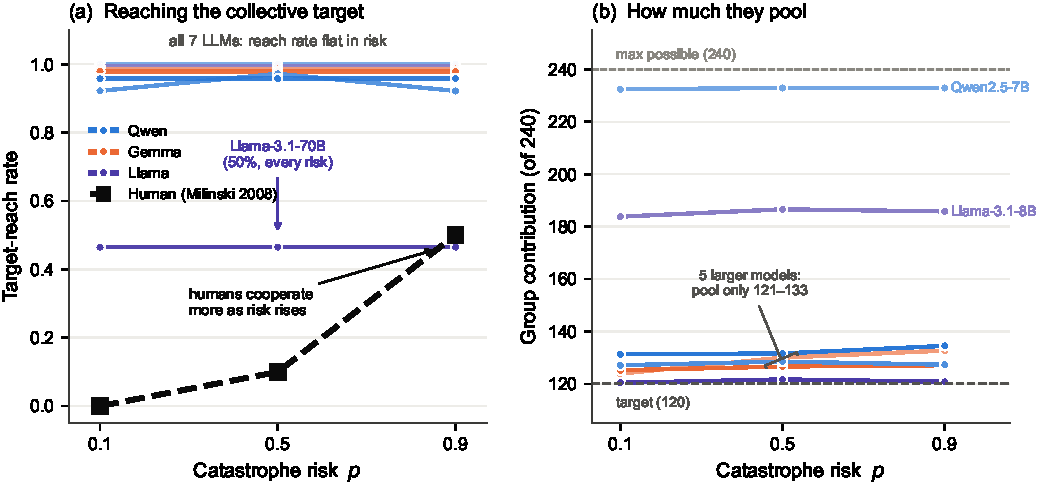
\includegraphics[width=\textwidth]{fig2_risk_insensitivity.pdf}
\caption{\textbf{No open-weight model reproduces the human risk response.} (a)~Target-reach rate against catastrophe risk for all seven open-weight models (colour denotes family; shade denotes size) and for humans (dashed). Every model's reach rate is flat in $p$; humans rise from $0\%$ to $50\%$. Llama-3.1-70B is flat at $50\%$. (b)~Group contribution (of a possible $240$) against risk. Contributions are essentially flat in $p$ (the one weak exception, Gemma-2-9B, is quantified in the text); the vertical spread reflects how economically each model plays, not risk sensitivity. In (a) five models sit exactly on $100\%$, so the curves are drawn with a small downward offset (at most $0.04$) purely so that all seven remain visible; no curve is drawn above its true value.}
\label{fig:risk}
\end{figure*}

\begin{figure}[t]
\centering
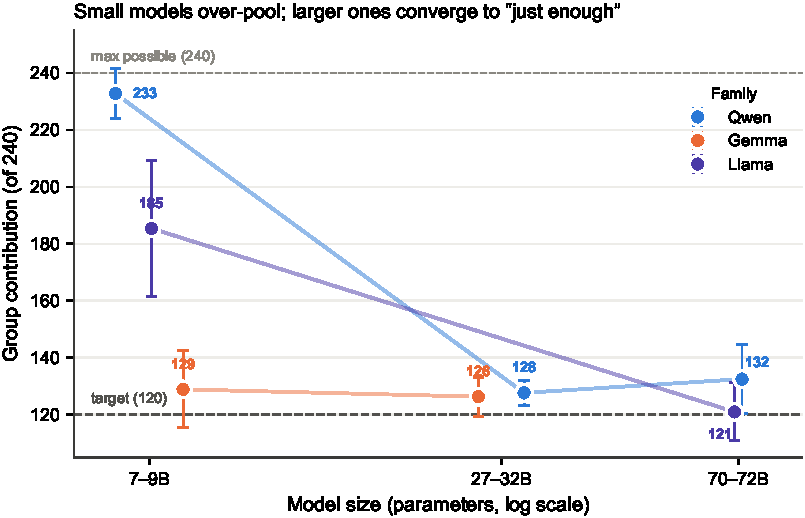
\includegraphics[width=\columnwidth]{fig3_economy_scaling.pdf}
\caption{\textbf{Small models over-pool; larger ones converge to ``just enough''.} Group contribution (of $240$) against model size on a logarithmic axis, connected within family. In every family the largest model pools far less than the smallest, but the decline is not strictly monotonic: Qwen2.5 falls to $127.6$ at 32B and rises again to $132.5$ at 72B. Error bars are standard deviations across games.}
\label{fig:economy}
\end{figure}

\subsection{What the prompt does that the incentive does not}
\label{sec:salience}
If a ninefold change in the probability of ruin barely moves these agents, what does? Three manipulations do, and none of them carries any information about payoffs, target or risk. They are the reason we describe the risk null as informative rather than merely negative: they are measured on the same games, under the same decoding, with the same dependent variable, so the comparison of magnitudes is internal.

The first is pure salience. Printing the running pool total in the prompt adds nothing an agent did not already have, since the total is a deterministic function of a history it is shown in full. It nevertheless moves behaviour by an order of magnitude more than risk does (figure~\ref{fig:salience}). Contributions fell by $95.3$ points for Qwen2.5-7B ($232.5\to137.2$, paired $P=6\times10^{-34}$), by $26.6$ for Llama-3.1-8B ($P=2\times10^{-17}$), by $8.2$ for Gemma-2-9B ($P=2\times10^{-6}$) and by $2.9$ for Qwen2.5-32B ($P=0.003$). The fifth model, Gemma-2-27B, shifted by the same $2.9$ points but not significantly ($P=0.16$); its target-reach rate nevertheless fell from $100\%$ to $67\%$, because it plays so close to the threshold that a shift too small to detect in contributions is large enough to change the outcome. The two smallest models, which over-contributed most when the total was hidden, are precisely the ones that correct hardest when it is shown.

The second is who is in the group. Replacing cooperative with selfish personas one agent at a time moves contributions monotonically and by a large margin: from all-cooperative to all-selfish, group contribution falls by $100.4$ points for Gemma-2-9B ($148.1\to47.7$, paired $P=6\times10^{-37}$), by $94.0$ for Llama-3.1-8B ($199.4\to105.4$, $P=3\times10^{-24}$), by $31.8$ for Qwen2.5-7B ($237.7\to205.9$, $P=4\times10^{-28}$) and by $112.4$ for GPT-5.4-nano in English. Even the smallest of these is more than three times the largest risk effect in the open-weight panel, and the largest is more than ten times it. What makes this manipulation informative is not only its size but its regularity. Group contribution falls almost perfectly linearly in the number of selfish agents (figure~\ref{fig:composition}(a)), with within-language $R^2$ of $0.95$ for both Gemma-2-9B and Llama-3.1-8B in English, $0.63$--$0.85$ elsewhere, and $0.89$ and $0.88$ in the two languages for GPT-5.4-nano. Each model is therefore summarised by two numbers, an intercept, the contribution of an all-cooperative group, and a slope, the cost of converting one cooperative agent into a selfish one: pooled across languages these are $146.5$ and $-16.6$ for Gemma-2-9B, $199.4$ and $-15.9$ for Llama-3.1-8B, $234.9$ and $-5.0$ for Qwen2.5-7B, and $210.5$ and $-18.8$ for GPT-5.4-nano in English.

That two-parameter description explains something that looks, on the raw reach curves, like three qualitatively different failure modes (figure~\ref{fig:composition}(b)). Gemma-2-9B's reach rate collapses immediately, halving at a single selfish agent and reaching zero by five. Llama-3.1-8B holds at or near $100\%$ through four selfish agents and then falls off a cliff, to $52\%$ at five and $28\%$ at six. Qwen2.5-7B never fails at all: it reaches the target in every one of its $420$ composition games, even when all six agents are told to be selfish. Yet all three obey the same linear law, and the difference is entirely where each line starts and how steeply it falls relative to a threshold that does not move. Gemma's line crosses $120$ at $1.6$ selfish agents, Llama's at $5.0$, GPT-5.4-nano's at $4.8$, and Qwen's only at $23.0$, that is, never, since the group has six members. Dramatic differences in apparent robustness are the arithmetic consequence of a linear response meeting a fixed threshold, not evidence of different strategies. It is also in these games that the decisive risk test of \S\ref{sec:results}\ref{sec:knifeedge} lives, and it is worth noting what the balanced cell shows directly: at three selfish agents against three cooperative ones, where groups are furthest from any ceiling, reach remains flat in risk for all three open-weight models and group contribution varies by less than $2.2$ points across the entire risk range. Making the group's fate genuinely uncertain does not make these agents attend to the probability that decides it.

The third is the language the prompt is written in, and in one model it is the largest single effect we measured anywhere. GPT-5.4-nano pooled $209.7$ in English and $62.9$ in Vietnamese, a paired difference of $146.8$ points of $240$ ($P=1\times10^{-16}$, $n=15$), and its target-reach rate went from $100\%$ to $0\%$. This is not a marginal shift in a model living near the threshold, as it was for Llama-3.1-70B: the Vietnamese groups pooled roughly half of the target, and $84$ of the $105$ Vietnamese composition games ended in a realised catastrophe. In Vietnamese the model begins below the threshold even when all six agents are told to be cooperative ($78.7$ of $240$), so the composition line never crosses $120$ at any composition and reach is floored at zero throughout (figure~\ref{fig:frontier}(b)), the mirror image of the ceiling censoring that limits the English cells. Placed on a common axis (figure~\ref{fig:frontier}(c)), the four manipulations separate by orders of magnitude for this model: catastrophe risk moves group contribution by $4.4$--$7.2$ points, group composition by $65.1$--$112.4$, and language by $146.8$. The one manipulation the game says should matter is the smallest of the four by a factor of nine to thirty-three.

Table~\ref{tab:effects} collects every effect in the study on the single scale that makes them comparable, points of the $240$ available, together with the channel each one travels through. Read down the table, the pattern that organises the paper is a single column: the manipulations delivered through the prompt move contributions by $95$ to $147$ points at their largest, the one delivered through the model itself by $105$, and the one delivered through the incentive structure by $0.97$ for eleven of the thirteen models. Only for the two models of \S\ref{sec:results}\ref{sec:toptier} does the incentive channel carry effects of the same order as the prompt channel.

\begin{table*}[t]
\centering
\caption{\textbf{What moves an agent, on one scale.} Change in group contribution
(of a possible $240$) produced by each manipulation. \emph{Channel} is how the
manipulation reaches the agent: through the incentive structure of the game, through
the text of the prompt, or through the model itself. The $\Delta$ column gives the
largest effect any model shows, with the range across models in the last column; the
one manipulation that carries information about payoffs is the smallest, for every
model except the two that solve the game. Every value is recomputed from the raw
per-game logs by \texttt{paper/revision/r6\_summary\_tables.py}.}
\label{tab:effects}
\footnotesize
\begin{tabular}{@{}llccll@{}}
\toprule
Manipulation & Channel & $\Delta$ contribution & $95\%$ CI & $P$ & Largest effect, and range \\
\midrule
Catastrophe risk, $p{=}0.1\!\to\!0.9$ & incentive & $+0.97$ & $[-2.2, +4.1]$ & $0.538$ & 11 models pooled, uncensored cells ($n{=}70$) \\
\quad the same, GPT-5.4-nano alone & incentive & $+7.5$ & $[-6.3, +21.2]$ & $0.263$ & cheap tier, uncensored ($n{=}15$) \\
\quad the same, the two EV models & incentive & $+118.2$, $+120.0$ & -- & -- & GPT-5.6-sol, Gemini-3.1-Pro \\
Printing the running pool total & prompt & $-95.3$ & -- & $<10^{-4}$ & Qwen2.5-7B ($2.9$--$95.3$, 5 models) \\
Group composition, $0\!\to\!6$ selfish & prompt & $-112.4$ & -- & -- & GPT-5.4-nano ($31.8$--$112.4$, 4 models) \\
Prompt language, Vietnamese $\to$ English & prompt & $+146.8$ & -- & $<10^{-4}$ & GPT-5.4-nano; reach $0\%\!\to\!100\%$ \\
Explicit reasoning, off $\to$ on & model & $-105.1$ & -- & -- & Grok-4.20; risk effect $+23.6\!\to\!+0.2$ \\
\bottomrule
\end{tabular}
\end{table*}


\begin{figure}[t]
\centering
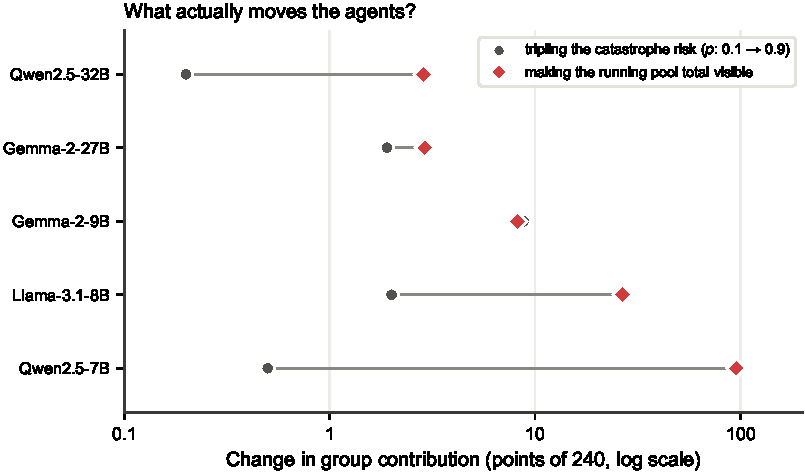
\includegraphics[width=\columnwidth]{fig7_salience.pdf}
\caption{\textbf{Salience beats incentive.} Absolute change in group contribution (of $240$, log axis) produced by two manipulations, for the five models run in both arms: tripling the catastrophe risk from $p=0.1$ to $p=0.9$ (grey circles, paired within seed) versus printing the running pool total in the prompt (red diamonds). The salience manipulation carries no information about payoffs, target or risk, yet dominates for four of the five models.}
\label{fig:salience}
\end{figure}

\begin{figure*}[t]
\centering
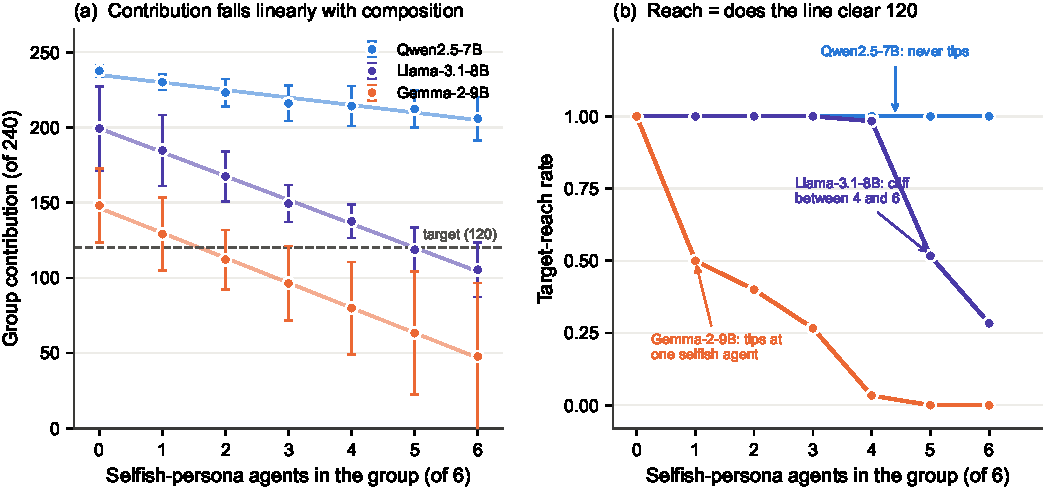
\includegraphics[width=\textwidth]{fig8_composition.pdf}
\caption{\textbf{Group composition is a linear engine against a fixed threshold.} (a)~Group contribution (of $240$) against the number of selfish-persona agents in the six-agent group, for the three open-weight models run in this study; lines are ordinary least-squares fits, points are cell means and error bars are standard deviations across games. The response is close to linear in every model ($R^2$ up to $0.95$ within language). (b)~The corresponding target-reach rates. The three apparently distinct failure modes, immediate collapse, a late cliff, and no failure at all, follow from where each model's line in (a) crosses the fixed target of $120$: at $1.6$, $5.0$ and $23.0$ selfish agents respectively.}
\label{fig:composition}
\end{figure*}

\begin{figure*}[t]
\centering
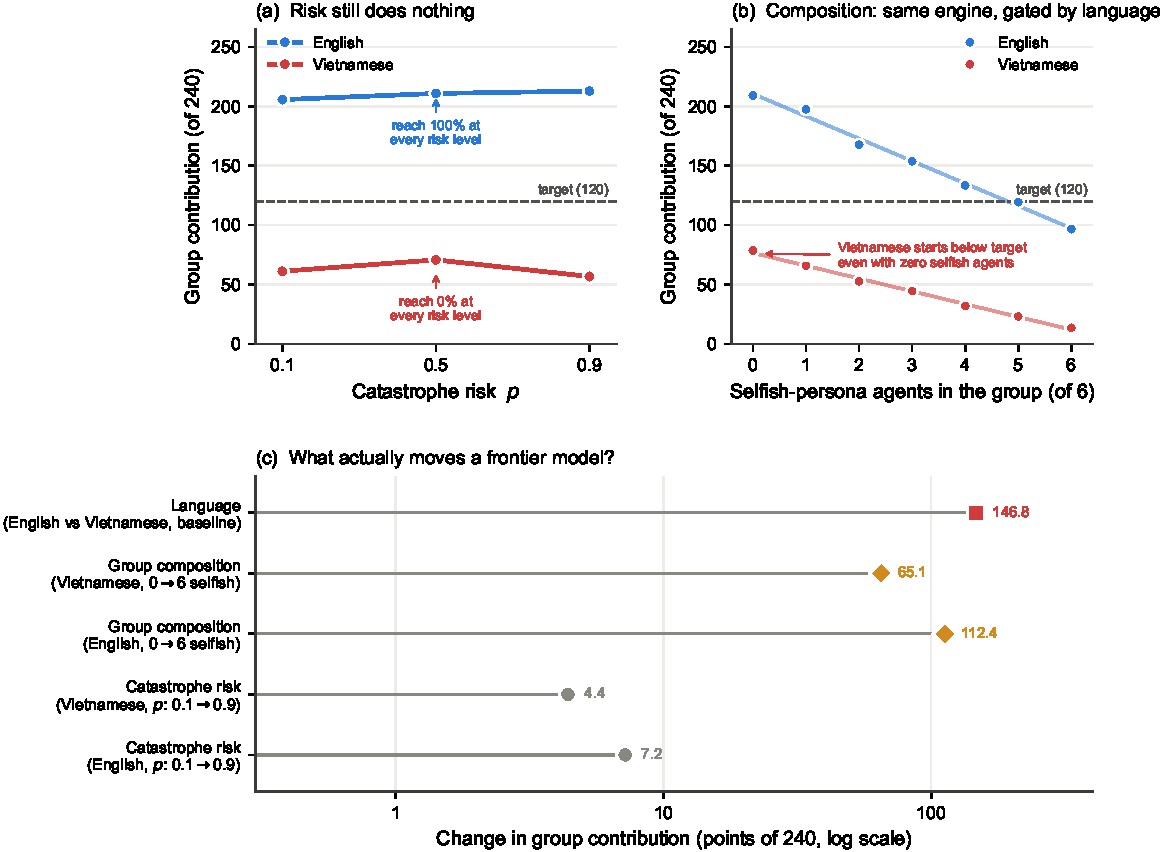
\includegraphics[width=\textwidth]{fig9_frontier.pdf}
\caption{\textbf{A cheap frontier model shows the open-weight pattern, and an extreme language effect.} GPT-5.4-nano, $30$ baseline and $210$ composition games. (a)~Group contribution against catastrophe risk, by language: flat in both, with English reaching the target in $100\%$ of games at every risk level and Vietnamese in $0\%$. (b)~The composition study shows the same near-linear engine as the open-weight models ($R^2=0.89$ and $0.88$ in the two languages), but the Vietnamese line starts below the target even with zero selfish agents, so it never crosses. (c)~The four manipulations on a common logarithmic axis. Risk is the smallest by a factor of nine to thirty-three.}
\label{fig:frontier}
\end{figure*}

\subsection{At the top of the frontier the null breaks, but only for two models}
\label{sec:toptier}
Everything to this point describes a panel that ignores the quantity the game is built around. Extending the panel to the top commercial tier does not sharpen that conclusion; it breaks it, and the break is the central result of the study.

Two of the six commercial models play the expected-value solution, and they play it almost exactly (figure~\ref{fig:toptier}(a)). Gemini-3.1-Pro contributed nothing whatsoever at $p=0.1$, a group total of $0.0$ of $240$ in all ten English games with zero variance, and then contributed exactly $120.0$, the target and not one unit more, in all twenty games at $p=0.5$ and $p=0.9$. GPT-5.6-sol did the same, pooling $1.6$ at $p=0.1$, $120.0$ at $p=0.5$ and $119.8$ at $p=0.9$. The English risk effect is $+120.0$ points of $240$ for Gemini-3.1-Pro, a difference between two constants for which no test is defined, and $+118.2$ for GPT-5.6-sol ($P=1\times10^{-22}$), roughly fourteen times the largest effect anywhere in the open-weight panel. Both hold up in Vietnamese, at $+119.6$ and $+74.2$ respectively.

These agents are not merely moving; they are winning. At $p=0.1$ an agent that contributes the target share ends with $20$ for certain, whereas one that withholds everything keeps $40$ and faces a one-in-ten lottery. Gemini-3.1-Pro's agents realised $32.0$ each and GPT-5.6-sol's $31.8$, against $20.0$ for Claude-Opus-5 and for Grok-4.20 with reasoning, the two top-tier configurations that paid exactly the target at that risk level, and less still for those that over-contributed ($19.7$ for Gemini-3.1-Flash-Lite, $7.1$ for Grok-4.20 without reasoning, $5.7$ for GPT-5.4-nano). The two models that walked away therefore earned $60\%$ more than the best-paid cooperator. The realised figures are below the expected $36$ because two of the ten shared lottery draws fell under $0.1$ and cost those groups everything, which is exactly what a risk-neutral agent accepts in exchange for the $90\%$ of games in which it keeps the full endowment. Since the draw schedule is the one part of the design we do not defend, it is worth removing it here rather than merely caveating it. Redrawing an independent uniform per game, $10{,}000$ times, over the contribution vectors exactly as observed, Gemini-3.1-Pro earns $36.0$ per agent ($95\%$ interval $[28.0,40.0]$) and GPT-5.6-sol $35.7$ ($[27.8,39.7]$), against a deterministic $20.0$ for the two top-tier configurations that paid the target, whose groups never face the lottery at all. The shared schedule cost these two models money: freed of it their advantage over the best-paid cooperator rises from $60\%$ to $79\%$, and even the $2.5$th percentile of their payoff distribution clears the cooperators' certain $20.0$. The behaviour is not merely thrift, either. At $p=0.5$, the point at which the two options have identical expected value, both models switch to cooperating and do so at exactly the minimum, contributing $120.0$; and at $p=0.9$ they cooperate again, GPT-5.6-sol missing the target by a single contribution in one of ten games ($118$ of $120$, giving a $90\%$ reach rate). The pattern across the three risk levels tracks the sign of the expected-value comparison, not a preference for either withholding or contributing, although \S\ref{sec:results}\ref{sec:pivot} shows that only one of the two models switches sign where a risk-neutral agent would.

The other four configurations do not. Claude-Opus-5 reached the target in all sixty of its games, with cell means spanning $120.0$ to $128.0$; its English risk effect of $+8.0$ points is highly significant ($P=3\times10^{-6}$) and behaviourally irrelevant, being $3\%$ of the board and never altering an outcome, and it falls to $+1.2$ ($P=0.41$) in Vietnamese. Grok-4.20 in its reasoning configuration is the most inert model in the entire study, contributing $120.0$ in twenty-nine of its thirty English games and $120.0$ in all thirty Vietnamese ones, for a risk effect of $+0.2$ and $+0.0$. Grok-4.20 with reasoning disabled contributes far more than it needs to, $197.2$ at $p=0.1$ rising to $220.8$ at $p=0.9$, and its $+23.6$-point slope is the largest at the top tier outside the two expected-value models, but it is not significant ($P=0.098$) and, more tellingly, it is a rise in the amount of over-contribution rather than a movement across any decision boundary: the model reaches the target in every game at every risk level, including the level at which reaching it is the wrong thing to do. At the cheap tier, Gemini-3.1-Flash-Lite moved $-1.8$ points, in the wrong direction, and GPT-5.4-nano $+7.5$.

The consequence for how such results should be read is visible in the reach rates (figure~\ref{fig:toptier}(b)). Target-reach at $p=0.1$ in English divides the panel perfectly and with nothing in between: $0\%$ for the two expected-value models and $100\%$ for every other configuration in the commercial panel. Had we run this study on any one top-tier model, as cost pressures normally dictate, we would have drawn a confident conclusion, and with probability one half it would have been the opposite of the truth.

\subsection{Capability is necessary but not sufficient, and reasoning buys thrift}
\label{sec:contrasts}
What distinguishes the two models that solve the game from the eleven that do not? Not the provider: the four top-tier models come from four different laboratories and divide two against two, so no vendor's alignment or training recipe accounts for the split. Not the presence of explicit deliberation: all four top-tier models are reasoning systems. And not capability alone, although capability is clearly involved. Figure~\ref{fig:toptier}(c) places all fourteen configurations on one axis, and the ordering is neither by size nor by tier nor by vendor. It is, as far as our design can tell, a property of the individual model.

Table~\ref{tab:axes} lays the panel out by family so that the two axes can be read apart. Within every family the larger or more expensive member is the thriftier one: Qwen2.5 falls from $232.7$ at 7B to $127.6$ at 32B, Llama from $185.4$ to $121.0$, Grok-4.20 from $225.1$ to $120.0$ when reasoning is enabled, GPT-5 from $136.3$ to $87.9$, Gemini-3.1 from $120.8$ to $80.1$. Thrift, in other words, is what capability reliably buys, and it is bought in every family we can compare. Risk sensitivity is bought in one family out of seven. The two columns are close to orthogonal: Gemini-3.1-Flash-Lite and Grok-4.20 with reasoning are as thrifty as models get without being risk-sensitive at all, both pooling within a point of the target and both reaching it at $p=0.1$ where reaching it is the wrong thing to do.

Two contrasts within the panel isolate what capability does and does not buy, and both are internal, changing one factor while holding the rest fixed. The first is the capability contrast, and it is the cleanest in the study because it holds the provider, the generation and the interface constant: Gemini-3.1-Flash-Lite and Gemini-3.1-Pro are the cheap and top tiers of one family, and their risk effects are $-1.8$ and $+120.0$ points respectively. The cheap model reaches the target in every game at every risk level; the expensive one refuses to at $p=0.1$ and then contributes exactly the target thereafter. Together with the observation that no model below the top commercial tier anywhere in our panel, open-weight or cheap-tier commercial, ever plays the expected-value solution, this supports a two-part claim that is stronger than either half alone: capability is necessary, since risk-responsive play appears only at the top tier, and capability is not sufficient, since half of the top tier does not exhibit it. The claim also answers the objection that most naturally meets a null result of this kind, namely that the models tested were simply not good enough.

The second contrast isolates explicit reasoning by toggling it within one base model. With reasoning disabled, Grok-4.20 pools $197.2$ at $p=0.1$ and $220.8$ at $p=0.9$ in English, and saturates in Vietnamese at $239.4$ of a possible $240$, tipping essentially the entire endowment into the pool every round; with reasoning enabled, the same model contributes $120.0$ at every risk level in both languages. Enabling reasoning is therefore worth $77.2$ points of $240$ at $p=0.1$ in English, and $105.1$ points pooled over all six cells, converting a model that gives away its endowment into one that pays the exact price of the target and keeps the rest. It is worth nothing at all in risk sensitivity: the risk effect falls from $+23.6$ to $+0.2$, and at $p=0.1$ the reasoning configuration still contributes $120$ where the expected-value solution contributes $0$. Deliberation, in this model, is spent on the question of how cheaply the target can be reached and not on the prior question of whether it is worth reaching. That is a sharper statement of the decoupling between capability and incentive-responsiveness than scale alone provided, because it is a within-model manipulation of the very faculty one would expect to produce the missing behaviour.

Finally, the risk-responsive models are not thereby human-like, and the difference matters for anyone proposing to use LLM agents as surrogates. Human groups in this dilemma reach the target in $0\%$, $10\%$ and $50\%$ of games as risk rises, a graded response that leaves most groups failing even when the catastrophe is nearly certain. Gemini-3.1-Pro and GPT-5.6-sol go $0\%$, $100\%$, $100\%$ (figure~\ref{fig:toptier}(b)): a step rather than a slope, agreeing with humans exactly where the expected-value solution and human behaviour happen to coincide, at $p=0.1$, and departing from them sharply everywhere else. The deviation from the human benchmark at the top tier is therefore an excess of decisiveness rather than a deficit of attention, which is the opposite failure mode from the one displayed by the other eleven models. Where each step actually falls is a question three risk levels cannot answer, and \S\ref{sec:results}\ref{sec:pivot} answers it on a five-point grid. \begin{table}[t]
\centering
\caption{\textbf{Economy of play and risk sensitivity are separate axes.} For each
configuration: how much the group pooled overall (of $240$; lower is thriftier), the
risk effect in English, and the target-reach rate at $p=0.1$, the risk level at which
reaching the target is the wrong thing to do. Within every family the larger or more
expensive member is thriftier; only in one family does it also become risk-sensitive.}
\label{tab:axes}
\small
\begin{tabular}{@{}llccll@{}}
\toprule
Family & Configuration & Pooled & $\Delta$ risk & Reach at $p{=}0.1$ & Reading \\
\midrule
Qwen2.5 & Qwen2.5-7B & $232.7$ & $+0.0$ & $100\%$ & profligate, risk-blind \\
 & Qwen2.5-32B & $127.6$ & $+1.4$ & $100\%$ & thrifty, risk-blind \\
 & Qwen2.5-72B & $132.5$ & $+2.4$ & $100\%$ & thrifty, risk-blind \\
\addlinespace[1pt]
Llama-3.1 & Llama-3.1-8B & $185.4$ & $+3.4$ & $100\%$ & profligate, risk-blind \\
 & Llama-3.1-70B & $121.0$ & $+0.4$ & $100\%$ & thrifty, risk-blind \\
\addlinespace[1pt]
Gemma-2 & Gemma-2-9B & $128.9$ & $+0.0$ & $100\%$ & thrifty, risk-blind \\
 & Gemma-2-27B & $126.3$ & $+3.8$ & $100\%$ & thrifty, risk-blind \\
\addlinespace[1pt]
Gemini-3.1 & Gemini-3.1-Flash-Lite & $120.8$ & $-1.8$ & $100\%$ & thrifty, risk-blind \\
 & Gemini-3.1-Pro & $80.1$ & $+120.0$ & $0\%$ & EV solution \\
\addlinespace[1pt]
GPT-5 & GPT-5.4-nano & $136.3$ & $+7.2$ & $100\%$ & profligate, risk-blind \\
 & GPT-5.6-sol & $87.9$ & $+118.2$ & $0\%$ & EV solution \\
\addlinespace[1pt]
Claude & Claude-Opus-5 & $124.6$ & $+8.0$ & $100\%$ & thrifty, risk-blind \\
\addlinespace[1pt]
Grok-4.20 & Grok-4.20 (no reasoning) & $225.1$ & $+23.6$ & $100\%$ & profligate, risk-blind \\
 & Grok-4.20 (reasoning) & $120.0$ & $+0.2$ & $100\%$ & thrifty, risk-blind \\
\bottomrule
\end{tabular}
\end{table}


Language shifts these agents too, and in model-specific directions that resist aggregation: Vietnamese leaves Gemini-3.1-Pro untouched ($+119.6$ against $+120.0$), degrades GPT-5.6-sol's expected-value play from $+118.2$ to $+74.2$ and inflates its standard deviation at $p=0.1$ from $1.6$ to $47.7$ as three of its ten Vietnamese groups revert to near-cooperative play, pooling $114$ and falling just short of the target, saturates Grok-4.20 without reasoning at the ceiling, and, in GPT-5.4-nano, inverts the outcome entirely. Four models, four directions: there is no single language effect to report.

\begin{figure*}[t]
\centering
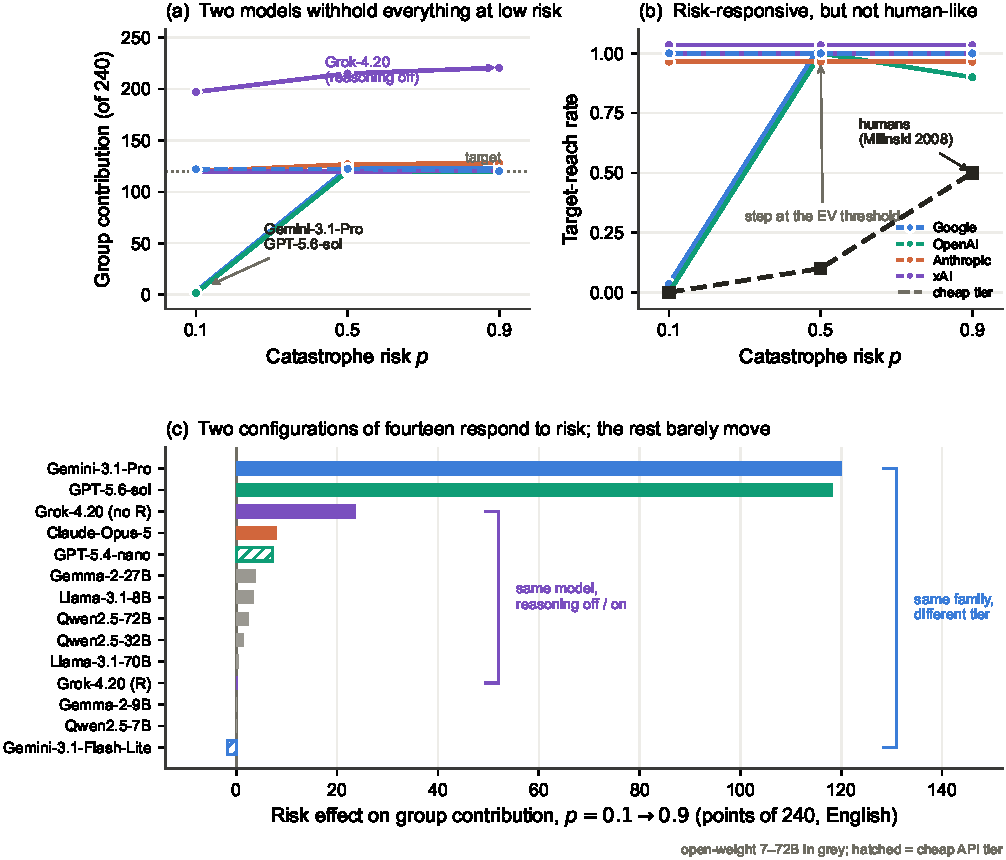
\includegraphics[width=\textwidth]{fig10_toptier.pdf}
\caption{\textbf{Risk sensitivity is a property of the model, not of the tier.} (a)~Group contribution (of $240$) against catastrophe risk in English for the six commercial models; solid lines are the top capability tier, dashed the cheap tier, colour denotes provider. Gemini-3.1-Pro and GPT-5.6-sol withhold everything at $p=0.1$ and then contribute exactly the target; the remaining configurations are flat. (b)~The corresponding target-reach rates against the human benchmark (black, dashed). The two responsive models form a step rather than a slope, more decisive than the graded human curve rather than blinder than it; figure~\ref{fig:pivot} locates the two steps on a five-point grid and shows that they do not coincide. (c)~Risk effect on group contribution across all fourteen configurations of the thirteen-model panel, sorted; open-weight models in grey, cheap commercial tiers hatched. The two bracketed pairs are the study's controlled contrasts: the same family at two capability tiers, and the same base model with explicit reasoning disabled and enabled. In (a) Gemini-3.1-Pro is drawn $3$ points high and in (b) three configurations are offset by at most $0.035$, purely so that coincident curves remain visible; the exact values are given in table~\ref{tab:headline}.}
\label{fig:toptier}
\end{figure*}

\subsection{Inside the game: the agents track the deadline, not what missing it costs}
\label{sec:trajectories}
Everything so far compares whole games. A game is ten decisions, though, and the within-game record answers a question the between-game comparison cannot: as evidence accumulates that the group will or will not reach the target, do the agents adjust, and does that adjustment depend on what failure would cost? We recomputed the $48{,}600$ baseline turns and the $88{,}200$ composition-study turns as trajectories to find out.

The first answer is visible without a test (figure~\ref{fig:trajectories}). For every configuration except the two that solve the game, the three risk curves lie on top of one another for all ten rounds; the separation that the whole-game analysis fails to find does not appear at any point inside the game either, so the null is not an artefact of aggregating over rounds. The second answer is more interesting, because the trajectories are not flat in \emph{time}. Three configurations show a marked endgame surge: Claude-Opus-5 and Qwen2.5-72B hold at exactly $2$ per agent through round seven and then climb, Qwen2.5-72B reaching the maximum of $4$ by round ten, and Llama-3.1-70B rises from round four before collapsing in the final round. These agents plainly do track something dynamic. What they track is the approach of the deadline, since the surge occurs at the same round and to the same height at every risk level.

Making that precise requires conditions in which the group's progress genuinely varies, which the baseline does not supply: almost every baseline group is on pace at almost every round. The composition study does, and there the natural quantity is the per-agent contribution still needed to finish on target, $\mathrm{need}(r)=(120-S_r)/(6\,(11-r))$ where $S_r$ is the pool before round $r$. Regressing an agent's contribution on $\mathrm{need}$, controlling for the agent's own mean contribution in earlier rounds and for round fixed effects, gives a coefficient that would be $1.0$ for an agent that exactly covers the remaining shortfall and $0$ for one that ignores it. Three of the four models sit slightly below zero ($-0.07$ to $-0.09$) and the fourth, Qwen2.5-7B, at $+0.44$: the agents are, at best, weak trackers of their own group's progress. Adding risk and its interaction with $\mathrm{need}$ asks the reviewer's question directly, whether an agent that is falling behind pushes harder when the catastrophe is more likely, and the interaction is indistinguishable from zero in all four models ($P=0.16$, $0.31$, $0.48$, $0.53$).

The same result survives a coarser and more legible test. Of the composition games, $548$ were behind pace at the start of round eight, meaning they needed more than $2$ per agent per round to finish on target. Comparing each group's mean contribution in rounds nine and ten against its own mean in rounds five to seven, the typical response to impending failure is not to push but to give up slightly: $-0.15$ at $p=0.1$, $-0.11$ at $p=0.5$ and $-0.06$ at $p=0.9$. The risk-dependence of that endgame push is $+0.12$ per unit probability (SE $0.06$, $P=0.051$), which across the full $p=0.1\to0.9$ sweep is $0.10$ of a contribution step per agent per round, or about $1.1$ points of $240$ over the two rounds in which it operates. Even at the moment when the catastrophe is closest and most avoidable, an agent facing near-certain ruin behaves within one-tenth of a step of an agent facing a one-in-ten chance.

\begin{figure*}[t]
\centering
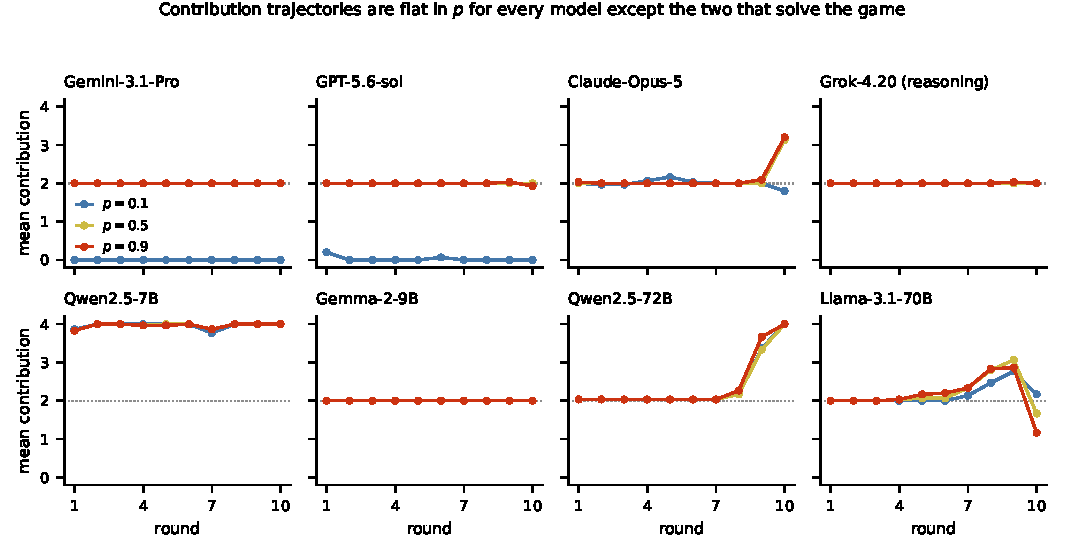
\includegraphics[width=\textwidth]{fig11_trajectories.pdf}
\caption{\textbf{Round-by-round contributions are flat in risk but not in time.} Mean per-agent contribution by round, in English, for the two expected-value models, two flat top-tier configurations and four open-weight models; colour denotes catastrophe risk. The dotted line marks the equal-split action of $2$. For every configuration except Gemini-3.1-Pro and GPT-5.6-sol the three curves are superimposed at every round, so the between-game risk null is not produced by averaging over rounds. Three configurations nevertheless show a clear endgame surge (Claude-Opus-5, Qwen2.5-72B, Llama-3.1-70B), which occurs at the same round and reaches the same height at all three risk levels: these agents track the deadline, not the cost of missing it.}
\label{fig:trajectories}
\end{figure*}

\subsection{Where the step falls: two models agree on a coarse grid and differ on a fine one}
\label{sec:pivot}
Three risk levels cannot say where a step is, and the question is not cosmetic. A step at $p=0.5$ is risk neutrality; a step below it is risk aversion; and the two are indistinguishable on a grid whose only interior point is the indifference point itself. We therefore returned to the four top-tier configurations and ran them in English at $p=0.3$ and $p=0.7$, ten independent games each, giving a five-point risk grid, $80$ games and $4{,}800$ agent-turns per configuration, again with no parse failures. The interval is chosen so that the expected-value comparison changes sign strictly inside it: at $p=0.3$ withholding is still worth an expected $28$ against a certain $20$, and at $p=0.7$ it is worth only $12$.

The two steps are not in the same place (figure~\ref{fig:pivot}). Gemini-3.1-Pro withholds at $p=0.3$ much as it does at $p=0.1$, pooling $4.2$ of $240$ and reaching the target in none of ten games, and then contributes exactly $120.0$ in every game at $p=0.5$, $0.7$ and $0.9$. Its step falls between $p=0.3$ and $p=0.5$, which is where risk neutrality puts it. GPT-5.6-sol has already turned by $p=0.3$: it pools $118.4$ and reaches the target in seven games of ten, at a risk level where the expected-value solution still says withhold. Choosing a certain $20$ over a gamble worth $28$ means giving up at least $8$ points, more than a quarter of the gamble's expected value, to avoid the gamble; treating $p=0.3$ as the point of indifference, that corresponds to a coefficient of relative risk aversion of about $0.5$. The model that looked risk-neutral on the coarse grid is mildly risk-averse on the fine one, and the agreement of the two models at $p=0.1$, $0.5$ and $0.9$ concealed a real difference in attitude rather than revealing a shared computation. This is the sharpest form of the paper's central caution: two models that are indistinguishable on three points of a design, and would have been reported as one phenomenon, separate as soon as the grid is refined.

The finer grid also sharpens the null and locates the study's only genuinely intermediate cell. Grok-4.20 with reasoning contributes $120.0$ at four of the five levels and $120.2$ at the fifth, with a standard deviation of zero everywhere but $p=0.9$: the two extra points buy no trace of a response that the coarse grid might have stepped over. Claude-Opus-5 reaches the target in every game at every level, but the amount it pools climbs monotonically, $120.0$, $120.6$, $126.8$, $128.0$, $128.0$, so its small risk effect is a widening margin of safety above a target it was always going to reach rather than a decision about whether to reach it. Against that background, GPT-5.6-sol at $p=0.3$ is the only cell anywhere in the top-tier panel in which the outcome genuinely varies: seven groups reached the target and three did not, with pooled totals spread over $114$, $120$ and $122$, against a standard deviation of exactly zero in most other top-tier cells. Whatever graded behaviour these models possess is confined to a band about one grid step wide around each model's own pivot, and is absent everywhere else.

\begin{figure}[t]
\centering
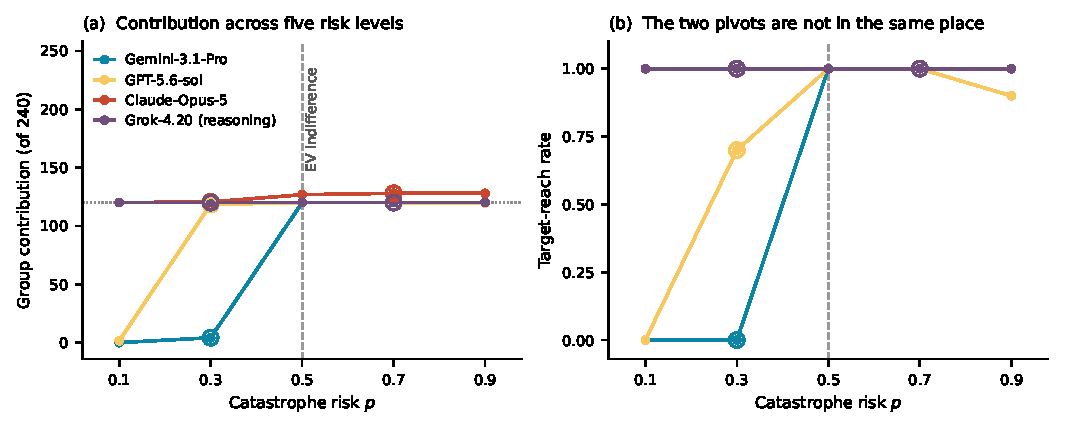
\includegraphics[width=\columnwidth]{fig12_pivot.pdf}
\caption{\textbf{Refining the risk grid separates two models that a three-point design merged.} The four top-tier configurations in English at five catastrophe risks, ten games per cell; open circles mark the two levels added after the original sweep. The dashed line is the expected-value indifference point $p=0.5$. (a)~Group contribution of a possible $240$; the dotted line is the target of $120$. (b)~Target-reach rate. Gemini-3.1-Pro steps between $p=0.3$ and $p=0.5$, where risk neutrality puts the step. GPT-5.6-sol has already stepped by $p=0.3$, reaching the target in seven of ten games at a risk level where withholding is worth an expected $28$ against a certain $20$, and is therefore risk-averse rather than risk-neutral. Grok-4.20 with reasoning is flat at the target across all five levels; Claude-Opus-5 always reaches it and merely widens its margin.}
\label{fig:pivot}
\end{figure}

\subsection{What the agents can and cannot do}
\label{sec:comprehension}
The behavioural deviation of the eleven risk-insensitive models might, in principle, be a failure of comprehension: perhaps they over-cooperated and ignored the risk because they did not grasp the rules or could not read the game. The in-situ probes rule this out for the open-weight panel. Accuracy on the \emph{Rules} axis was uniformly high, from $93.8\%$ for Llama-3.1-8B to $100\%$ for the five largest models, and accuracy on the \emph{Time} axis, reading specific events from the history, ranged from $82\%$ to $99\%$ (figure~\ref{fig:comprehension}). One probe asked the model to state the catastrophe probability of the game it was playing, and every model answered almost always correctly: $98.1\%$ for Qwen2.5-7B, $91.4\%$ for Llama-3.1-8B and $100\%$ for the other five (figure~\ref{fig:mechanism}(b), upper curve). We are deliberately modest about what this shows. The decision prompt prints the catastrophe probability verbatim, so the probe is a retrieval task, and these models copy printed values at ceiling throughout our data. It establishes that the risk was legible in the context the agent decided from, which is worth establishing since it rules out the possibility that the number was lost or garbled, but it does not show that the agent represented the risk as a decision-relevant quantity, and it cannot distinguish an agent that weighed the risk and set it aside from one that never entered it into a calculation at all.

The only axis on which the models struggled was \emph{State}, the current cumulative situation, and the reason is specific and revealing. When we asked for a quantity that was printed verbatim in the prompt, for example a player's own remaining money, accuracy was high for every model: under the same hidden-pool prompt used for the comparison below, five of the seven answered at or within a fraction of a point of ceiling, and Qwen2.5-7B scored $89.0\%$. The exception is Llama-3.1-8B, at $68.8\%$ overall and only $46.0\%$ in English; that model cannot reliably read the printed value either, so it is a poor test of the dissociation, and the contrast below should be read from the other six. When we asked for the same kind of quantity that had to be \emph{summed} across rounds, namely the running pool total while it was hidden from the prompt, small models collapsed: Qwen2.5-7B answered correctly only $14.3\%$ of the time and Llama-3.1-8B only $9.8\%$, even though both could read a printed value almost perfectly (figure~\ref{fig:mechanism}(a)). That the failure is arithmetic rather than perceptual is confirmed by the A/B manipulation: when the same pool total was printed rather than hidden, accuracy jumped to $92$--$100\%$ across the board. Reading, in other words, is not adding. This cumulative-addition deficit is a property of small models that scale largely removes. Accuracy on the hidden pool total rose steeply, if not perfectly monotonically, with size: $14.3\%$ and $9.8\%$ for the 7B and 8B models, $21.2\%$, $61.5\%$ and $43.5\%$ for the 9B, 27B and 32B models, and $81.7\%$ and $88.2\%$ for the 70B and 72B models (figure~\ref{fig:mechanism}(b), lower curve); the two local reversals fall between families rather than within them. The juxtaposition in figure~\ref{fig:mechanism}(b) is the one that matters: knowledge of the risk is flat and near-perfect across the whole size range, while the ability to track cumulative state climbs steeply with scale. By 70--72B the models both know the risk and can add the pool, and they still ignore the risk.

Language separates these two capacities cleanly (figure~\ref{fig:language}). Behaviourally, the two languages produced identical target-reach rates for five of the seven open-weight models; Qwen2.5-32B dipped slightly ($100\%$ in English versus $93.3\%$ in Vietnamese) and Llama-3.1-70B collapsed outright, from $100\%$ to $0\%$. In comprehension, language left rule and risk knowledge essentially untouched, with Rules accuracy differing by under one percentage point between languages and the risk probability read correctly in both, but it selectively attacked the arithmetic: State accuracy fell from $73.6\%$ in English to $61.8\%$ in Vietnamese, an almost twelve-point drop. The damage was concentrated in the middle of the range rather than at the bottom, with Gemma-2-9B losing the most ($87.8\%$ to $56.4\%$, $31.5$ points) while the two models that were already worst at cumulative addition had the least left to lose (Qwen2.5-7B $13.6$ points, Llama-3.1-8B $11.3$ points) and Llama-3.3-70B was unaffected (Vietnamese in fact $0.8$ points higher). Language, then, changes what these models can compute far more than what they know. We emphasise that this gate is available only for the open-weight panel: the commercial models, including the two that solve the game, carry no comprehension data, so we can say that the eleven risk-insensitive open-weight and cheap models did not misunderstand the game, and we cannot say by what internal route the two responsive models arrive at the expected-value solution.

\begin{figure}[t]
\centering
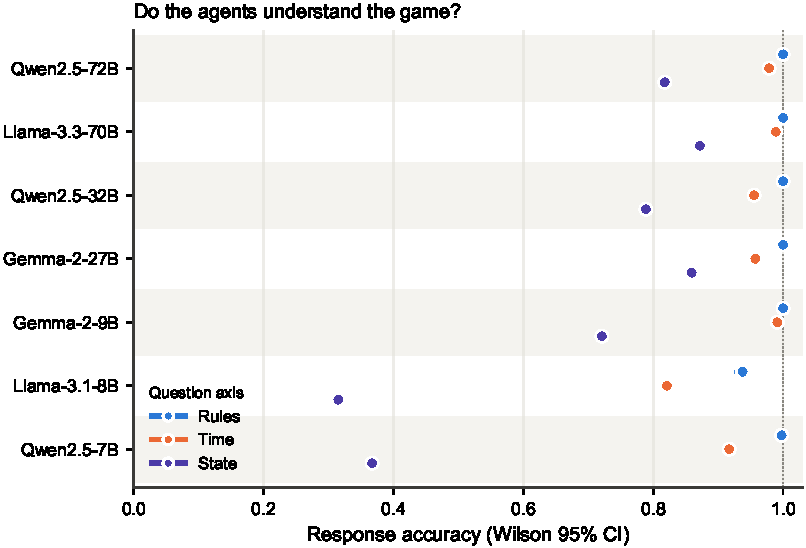
\includegraphics[width=\columnwidth]{fig4_comprehension_category.pdf}
\caption{\textbf{Comprehension by question axis.} Response accuracy (dots) with Wilson $95\%$ confidence intervals for each model, ordered by size (smallest at the bottom), on the Rules, Time and State axes; alternating bands group the three dots belonging to one model, and with $2{,}880$--$28{,}200$ probes per point the intervals are narrower than the markers. Rules is at ceiling and Time is high ($82$--$99\%$) for all models; State (cumulative situation) is the only axis that varies widely, and it improves broadly with scale.}
\label{fig:comprehension}
\end{figure}

\begin{figure*}[t]
\centering
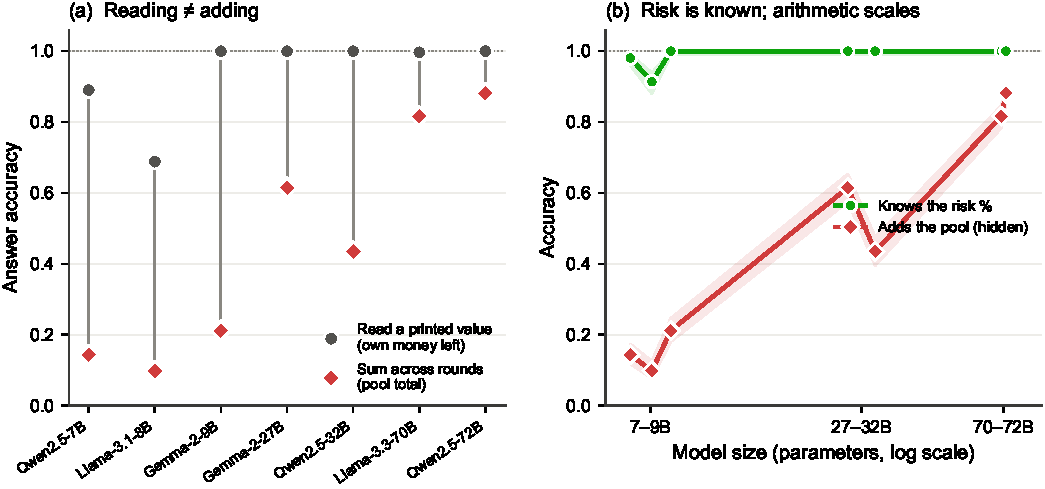
\includegraphics[width=\textwidth]{fig5_mechanism.pdf}
\caption{\textbf{The gap is arithmetic, and it closes with scale.} (a)~Under the default hidden-pool prompt, accuracy on a value the agent can read straight off the prompt (its own money left, grey circles) versus a value it must sum across rounds (the pool total, red diamonds). Small models can read but cannot add. The same-question control is the A/B in the text: printing the pool total lifts accuracy on that identical question to $92$--$100\%$. (b)~Knowledge of the catastrophe probability (green) is flat and near-perfect across the size range, whereas the ability to sum the hidden pool (red) rises steeply with scale. Even where both are near-ceiling, behaviour remains risk-insensitive. Bands are Wilson $95\%$ intervals.}
\label{fig:mechanism}
\end{figure*}

\begin{figure*}[t]
\centering
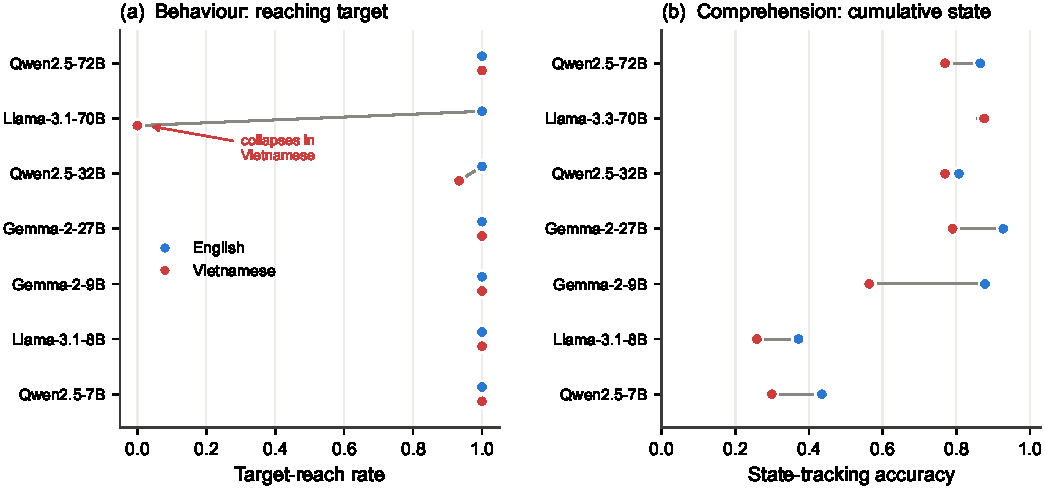
\includegraphics[width=\textwidth]{fig6_language.pdf}
\caption{\textbf{English versus Vietnamese.} (a)~Target-reach rate in each language for the seven open-weight models, the two points of a pair offset vertically so that coincident values stay visible. Behaviour is identical across languages for five of the seven; Qwen2.5-32B dips slightly ($100\%$ to $93.3\%$) and Llama-3.1-70B collapses from $100\%$ to $0\%$ in Vietnamese. (b)~Cumulative-state accuracy in each language. Vietnamese selectively degrades the arithmetic; the largest loss is Gemma-2-9B ($31.5$ points), while the weakest adders have least left to lose and Llama-3.3-70B is unaffected.}
\label{fig:language}
\end{figure*}

\begin{table*}[t]
\centering
\caption{\textbf{Headline results per model.} Behavioural quantities pooled over risk and language ($60$ games per configuration; $30$ for GPT-5.4-nano): target-reach rate and group contribution (of $240$). The risk column gives the change in group contribution from $p=0.1$ to $p=0.9$ in English, the study's central quantity. The composition column gives the change from an all-cooperative to an all-selfish group, for the four models run in that study. Comprehension quantities come from the in-situ probes: accuracy at stating the catastrophe probability (\emph{risk knowledge}) and at summing the hidden pool (\emph{cumulative arithmetic}); the commercial panel carries none. Human target-reach rates rise from $0\%$ to $10\%$ to $50\%$ with risk.}
\label{tab:headline}
\small
\begin{tabular}{@{}llcccccc@{}}
\toprule
& & \multicolumn{2}{c}{Behaviour} & \multicolumn{2}{c}{Effect on contribution} & \multicolumn{2}{c}{Comprehension} \\
\cmidrule(lr){3-4}\cmidrule(lr){5-6}\cmidrule(lr){7-8}
Model & \shortstack[l]{Size or\\tier} & Reach & \shortstack{Contri-\\bution} & \shortstack{$\Delta$ risk\\(en)} & \shortstack{$\Delta$ 0$\to$6\\selfish} & \shortstack{Risk\\knowledge} & \shortstack{Cumulative\\arithmetic} \\
\midrule
\multicolumn{8}{@{}l}{\emph{Open-weight, served locally}}\\
Qwen2.5-7B    & 7B  & $100\%$  & $232.7$ & $+0.0$  & $-31.8$  & $98.1\%$ & $14.3\%$ \\
Llama-3.1-8B  & 8B  & $100\%$  & $185.4$ & $+3.4$  & $-94.0$  & $91.4\%$ & $9.8\%$  \\
Gemma-2-9B    & 9B  & $100\%$  & $128.9$ & $+0.0$  & $-100.4$ & $100\%$  & $21.2\%$ \\
Gemma-2-27B   & 27B & $100\%$  & $126.3$ & $+3.8$  & --       & $100\%$  & $61.5\%$ \\
Qwen2.5-32B   & 32B & $96.7\%$ & $127.6$ & $+1.4$  & --       & $100\%$  & $43.5\%$ \\
Llama-3.1-70B & 70B & $50\%$   & $121.0$ & $+0.4$  & --       & $100\%$\textsuperscript{*} & $81.7\%$\textsuperscript{*} \\
Qwen2.5-72B   & 72B & $100\%$  & $132.5$ & $+2.4$  & --       & $100\%$  & $88.2\%$ \\
\midrule
\multicolumn{8}{@{}l}{\emph{Commercial, hosted}}\\
GPT-5.4-nano            & cheap & $50\%$\textsuperscript{\dag} & $136.3$\textsuperscript{\dag} & $+7.2$   & $-112.4$\textsuperscript{\ddag} & -- & -- \\
Gemini-3.1-Flash-Lite   & cheap & $100\%$  & $120.8$ & $-1.8$   & -- & -- & -- \\
Claude-Opus-5           & top   & $100\%$  & $124.6$ & $+8.0$   & -- & -- & -- \\
Grok-4.20 (reasoning)   & top   & $100\%$  & $120.0$ & $+0.2$   & -- & -- & -- \\
Grok-4.20 (no reasoning)& top   & $100\%$  & $225.1$ & $+23.6$  & -- & -- & -- \\
GPT-5.6-sol             & top   & $65\%$   & $87.9$  & $\mathbf{+118.2}$ & -- & -- & -- \\
Gemini-3.1-Pro          & top   & $66.7\%$ & $80.1$  & $\mathbf{+120.0}$ & -- & -- & -- \\
\bottomrule
\end{tabular}\\[2pt]
{\footnotesize \textsuperscript{*}Llama-3.3-70B in the comprehension study.
\textsuperscript{\dag}Pooled over language; the pooled figure is a mixture of $100\%$ reach in English and $0\%$ in Vietnamese and should not be read as a knife-edge strategy (\S\ref{sec:results}\ref{sec:salience}).
\textsuperscript{\ddag}English; the Vietnamese figure is $-65.1$ from a starting point already below the target.
For GPT-5.6-sol and Gemini-3.1-Pro the sub-unity reach rate is the expected-value solution rather than a failure: both reach the target in $100\%$ of games at $p=0.5$ and $p=0.9$ and in $0\%$ at $p=0.1$, where withholding is worth more (\S\ref{sec:results}\ref{sec:toptier}).}
\end{table*}

\section{Discussion}
\label{sec:discussion}

The central result of this study is a dissociation measured under one game. Across seven open-weight models spanning an order of magnitude of scale, two cheap commercial models and two of the four top-tier ones, a ninefold increase in the probability of losing everything moves cooperation by no consequential amount, and by an amount statistically indistinguishable from zero wherever the outcome was free to move, while three manipulations that carry no information about payoffs, target or risk each move it by tens to over a hundred points: displaying a number the agent already had the information to compute, changing which dispositions are named in the six prompts, and changing the language those prompts are written in. The unifying observation for those eleven models is that all three manipulations that work are delivered through the prompt, and the one that does not work is delivered through the incentive structure. It is not that these agents fail to respond to their situation, since they respond vigorously, and in the normatively sensible direction, to being told who they are and to being shown the state of play. It is that the channel through which a game communicates stakes, namely the consequences attached to outcomes, is the channel they attend to least. An agent that adjusts its contribution by a hundred points when a neighbouring prompt says ``selfish'', and by one point when its own probability of losing everything rises from one-in-ten to nine-in-ten, is not weighing costs and benefits in any recognisable sense.

The other two models weigh them precisely. Gemini-3.1-Pro and GPT-5.6-sol give away nothing when the catastrophe is unlikely, pay exactly the target when it is not, and are paid $60\%$ more for the difference. This is not a small quantitative improvement on the panel; it is a categorical change in what governs the behaviour, and it is what converts our null from a claim about language models into a claim about most language models. Any evaluation of this kind that had been run on one model, as budget normally dictates, would have reported one of two opposite conclusions with equal confidence, and our own earlier draft, built on a single cheap frontier model, reported the wrong one. The methodological lesson generalises well beyond this game: where a behaviour is a property of individual systems rather than of the technology, the sample size that matters is the number of models, and it is the axis on which behavioural evaluations of LLMs are most systematically underpowered.

What the split is not is as informative as what it is. It is not a provider effect, since four top-tier models from four laboratories divide two against two. It is not the presence of explicit reasoning, since all four are reasoning systems and the most inert configuration in the entire study is a reasoning one. It is not capability alone, although capability is a precondition: no model below the top commercial tier anywhere in the panel plays the expected-value solution, and the cleanest single contrast we have, between two members of one family and generation that differ only in tier, separates a $-1.8$-point risk response from a $+120.0$-point one. Capability is therefore necessary and not sufficient, which is the formulation that survives the objection most often raised against nulls of this kind, that the models tested were simply not good enough. Half of the best models available to us were, in this precise sense, not good enough, and it was not because they could not read the game.

The reasoning contrast sharpens the same point into a mechanism. Disabling explicit reasoning in Grok-4.20 raises its contribution from $120.0$ to $197.2$ at $p=0.1$ and to $239.4$ of $240$ in Vietnamese; enabling it returns the model to paying the exact price of the target. Deliberation is worth $105.1$ points of $240$ in efficiency and nothing at all in risk sensitivity: the risk slope falls from $+23.6$ to $+0.2$ and the model still contributes $120$ at the risk level where the expected-value solution contributes $0$. The faculty is spent on the question of how cheaply the goal can be reached, never on the prior question of whether the goal is worth reaching. Read against the open-weight panel, where scaling from 7B to 72B improves cumulative arithmetic from near-chance to near-ceiling~\cite{wei2022emergent} while leaving the behavioural prior untouched, the picture is consistent: competence and the disposition to act on incentives are separate axes, and moving along the first does not move an agent along the second. Something else does, and our design localises it only to the individual model.

We are equally careful about what the risk-responsive models do not show. They do not reproduce human behaviour; they overshoot it. Human groups reach the target in $0\%$, $10\%$ and $50\%$ of games as risk rises, whereas Gemini-3.1-Pro and GPT-5.6-sol go $0\%$, $100\%$, $100\%$, a step where the human response is a slope. The two failure modes we observe are therefore opposite in direction and equally disqualifying for surrogate use: eleven models cooperate when humans would not, and two coordinate perfectly at a risk level where half of human groups still fail. Nor can we show that these two models compute the expected value, and the five-point grid makes that reservation concrete rather than merely prudent. On three risk levels their behaviour coincided exactly with what a risk-neutral agent would do; on five it does not, because GPT-5.6-sol switches a full grid step early and pays a risk premium of at least a quarter of the gamble's expected value to do so. Coincidence with a normative solution is thus an artefact of grid resolution as much as a property of the agent, and it is the resolution, not the coincidence, that a reader should interrogate first. The hosted interface returns the chosen contribution and no deliberation trace, so distinguishing a calculation from a well-generalised heuristic still requires a design that interrogates the agent directly, and it remains the natural next study.

The composition study adds a lesson about how such systems fail. The response to composition is close to linear and the threshold is fixed, so whether a group succeeds is determined by where a straight line crosses a horizontal one. This makes collective failure both highly predictable and highly discontinuous: two models with similar per-agent behaviour can have completely different tipping points, and a model can appear perfectly robust across a wide range of compositions and then fail almost completely within one further step. Qwen2.5-7B never failed in $420$ composition games not because it resists selfish framing better than the others, since its slope is genuinely negative, but because its intercept is so high that six selfish agents are not enough to bring it down. Robustness, here, is a property of the margin between an intercept and a threshold, not of anything one would call resilience. For anyone deploying a fleet of agents to a shared quantitative goal, the observable per-agent quantities are the intercept and the slope, and these, rather than the observed success rate, determine how much adverse composition the system can absorb.

These findings connect to prior work whose picture is more mixed than a single summary allows. Some studies report LLMs that are markedly more cooperative and more forgiving than humans in repeated dilemmas~\cite{fontana2024nicer,phelps2023investigating}; others report the opposite temperament, with GPT-4 retaliating unforgivingly after a single defection~\cite{akata2023playing}, and most models failing to sustain a shared resource without explicit institutional scaffolding~\cite{piatti2024cooperate}. Our panel suggests that this disagreement may be less a matter of task or of prompt than of which model was to hand: within a single fixed game we obtain both temperaments, and the dividing line runs between models of nominally the same class. That reading is reinforced by the surveyed breadth of the field~\cite{feng2024survey} and by how easily a single-model study reaches a confident and opposite conclusion: Yao and colleagues, testing one model in non-zero-sum games, find cooperation driven by explicit fairness reasoning~\cite{yao2026competition}, a temperament our panel produces in some members and not others.

Three lines of recent work bear on the specific dissociation we report. The first concerns what changes to the game's own structure can buy. CoopEval compares four families of cooperation-sustaining mechanism across four dilemmas and finds contracting and mediation clearly more effective than repetition or reputation, with repetition-induced cooperation collapsing when co-players vary~\cite{tewolde2026coopeval}. The most direct precursor to the present study is the payoff-scaled prisoner's dilemma of~\cite{huynh2025understanding}, built on the same framework and by an overlapping group, which isolates sensitivity to incentive \emph{magnitude} and finds cooperation that does respond to it, together with cross-linguistic divergence of the kind we report here. Read together, the two studies bound where incentive sensitivity survives, and the present result is the boundary case. Incentive levers do move LLM agents, but not all levers transfer across game families: where scaling the return in a public-goods game raises cooperation, scaling the probability of ruin in a threshold game leaves eleven of thirteen models where they were. What distinguishes the two is not size of stake but the fact that risk enters only through an expectation the agent must form for itself, whereas a changed payoff enters the arithmetic of every round.

The second concerns deliberation. Li and Shirado show that reasoning models consistently reduce cooperation and norm enforcement across six economic games, a pattern they name spontaneous giving and calculated greed~\cite{li2025spontaneous}. Our within-model toggle agrees on the sign and sharpens the interpretation: enabling reasoning in Grok-4.20 is worth $105$ points of thrift, moving the model from giving away its endowment to paying the exact price of the target, and is worth nothing whatever in risk sensitivity. Deliberation, at least here, is spent on the cost of reaching a goal and never on whether the goal is worth reaching, which is a more specific finding than reduced prosociality and explains why more reasoning need not produce more incentive-aligned behaviour. Relatedly, MoralSim embeds the prisoner's dilemma and the public-goods game in morally charged contexts and finds substantial between-model variation with no model consistently moral~\cite{backmann2025ethics}; the between-model variance we find on a purely material manipulation suggests that such variation is not confined to moral framings.

The third concerns how much of LLM behaviour is carried by the prompt rather than by the game. Communication and framing modulate multi-agent LLM behaviour strongly and in language-dependent ways~\cite{buscemi2025strategic,madmoun2025communication}, and the declared identity of the opponent shifts cooperation even for human players facing an LLM~\cite{jiang2025trust}. Our contribution to that thread is a magnitude comparison held to one game and one dependent variable: prompt-side factors do not merely modulate behaviour alongside the incentive structure, they dominate it, by one to two orders of magnitude, for most of the models we tested (table~\ref{tab:effects}). The composition result also bears on the practice of persona-conditioning LLMs to stand in for heterogeneous human populations~\cite{argyle2023out,aher2023using}: personas do move behaviour substantially and monotonically, which is encouraging for that practice, but in our data they move it far more reliably than the game's own incentives do for most models, which means a persona-conditioned population may reproduce the distribution of stated dispositions while badly misrepresenting how that population would respond to changing stakes. Methodologically, the study extends the in-situ understanding-check paradigm from the two-player prisoner's dilemma~\cite{fontana2024nicer} to an $N$-player threshold game and shows that a single well-chosen probe, can the model state the risk it faces, separates one important confound from a behavioural claim.

Our results carry four practical implications. First, LLM agents are unreliable surrogates for humans in risk-structured collective decisions, and they are unreliable in two distinct ways: most of them predict near-certain cooperation at a level of risk where human groups in fact reach the target only half the time, while the most capable of them predict perfect coordination where humans are divided. Second, an agent's incentive-responsiveness cannot be inferred from its competence, from its vendor, or from its price tier; it has to be measured, and measured on the specific model to be deployed, because two models from the same family and generation differ here by the width of the board. Third, group composition is both the most reliable lever and the most treacherous one, since it moves behaviour linearly and predictably but converts into success or failure through a threshold, so systems can look robust right up until they are not. Fourth, language is not neutral: deploying the same model in a lower-resource language preserved its factual knowledge of the game but degraded its quantitative reasoning, and its behavioural consequences ran in four different directions across four models, from no effect at all to a complete inversion of the outcome. There is no single multilingual correction to apply.

\label{sec:limits}
Several limitations bound these conclusions, and the first is severe enough that we place it ahead of the others. Our decision prompt names the equal-split solution. An agent that contributes 2 is therefore consistent with a cooperative disposition, with plain instruction-following, or with anchoring on the only number the prompt offers, and this study cannot tell them apart. The evidence that this is not hypothetical is in our own data: Gemma-2-9B produced a group total of exactly $120.0$ in all thirty English games, Gemma-2-27B did the same in Vietnamese, and at the top tier Grok-4.20 with reasoning and both risk-responsive models land on exactly $120$ in all but two of the games in which they cooperate at all. Any claim in this paper about cooperative dispositions should be read as a claim about behaviour under a prompt that supplies a focal action; the clean experiment removes the hint and re-runs, and we regard that as the necessary sequel rather than an optional extension.

What the existing data can settle is the narrower and more dangerous version of the objection, that the anchor is what produces the risk null. It is not, and the reason is that the anchor's grip is neither uniform nor strong. Across the fourteen configurations the probability of taking the focal action ranges from $0.054$ for Qwen2.5-7B to $1.000$ for Grok-4.20 with reasoning, so five configurations take it in fewer than a third of their turns. If anchoring produced the null, the models that ignore the anchor would be free to respond to risk and should show the larger risk effects. They do not: the correlation between how often a model takes the focal action and the magnitude of its risk response is $-0.06$ across the panel, and the two extremes are a model that almost never takes the anchor and has a risk effect of exactly $0.0$ (Qwen2.5-7B) and a model that always takes it and has a risk effect of $+0.2$ (Grok-4.20 with reasoning). The same conclusion follows from the manipulations that do work: an anchor that yields by $15$ percentage points to one sentence of persona and by $10$ to a change of language, while holding to within $4$ points across a ninefold change in the probability of ruin, is not a constraint strong enough to be the cause of the null. Finally, the hint cuts the other way for the risk-responsive models, since it makes their behaviour at $p=0.1$ harder rather than easier to produce: withholding everything requires overriding the focal action the prompt supplies, and Gemini-3.1-Pro does so in $100\%$ of its turns there and GPT-5.6-sol in $98.8\%$, which is why we regard the $0.0$ contributions as the most informative single number in the study.

The remaining limitations are of coverage and implementation. The commercial panel is observed only in the baseline design: it carries no comprehension probes, so we cannot gate its behaviour on understanding as we do for the open-weight models, and no composition study, so the linear-engine description is established at 7--9B and in one cheap commercial model, not at the top tier. Those models are also served through third-party interfaces: temperature and the output cap were ours to set and were set, but $\mathrm{top}\_p$ was left at provider defaults, the honouring of a per-turn seed is not guaranteed by any of the four providers, and no deliberation trace is returned, so their games are unpaired with the open-weight arm and we observe outcomes rather than process. Their near-determinism cuts both ways: with $20$ of the $44$ ten-repetition commercial cells showing exactly zero variance across their ten games, effects are estimated with unusual precision but the uncensored-cell test that anchors the open-weight analysis cannot be run there at all, which is why the top-tier contrasts are between models rather than within them. Ten repetitions per cell is enough to establish a $120$-point difference and not enough to characterise the tail of a rare behaviour. The refined risk grid inherits both restrictions: it was run in English only and at the top tier only, so it locates GPT-5.6-sol's pivot at or below $p=0.3$ without bracketing it more tightly, and it says nothing about whether the cheap tier or the Vietnamese prompt would move either pivot. The persona-to-seat permutation is deterministic rather than uniformly random and is not perfectly balanced across seats, so we make no claims about position effects. The groups were homogeneous in model and mute, since all six agents were the same model and could not communicate, whereas human cooperation is shaped by heterogeneity and cheap talk, so our estimates speak to a specific controlled regime rather than to open multi-agent interaction. The catastrophe was a single end-of-game lottery drawn from a schedule shared across conditions, which makes realised disaster rates uninformative and is why we treated reach rate and contribution as the primary dependent variables; it does not, however, contaminate behaviour, since the draw is made after the last decision and never shown to any agent, and neither repetition index nor a previous repetition's catastrophe predicts contribution (\S\ref{sec:methods}). Two confounds bound the scaling claim in particular: the 70B and 72B models were served with activation-aware weight quantisation while the smaller ones were not, so scale is not a perfectly clean manipulation, and the Milinski design is old and widely reproduced, so it is likely present in every model's training corpus, meaning an agent may partly be recognising a familiar task rather than reasoning about it afresh. That last concern is sharpest exactly where our new result lives, since the most capable models are the most likely to have absorbed the literature, and it cannot be settled without a novel isomorphic game. Finally, we studied instruction-tuned models only, so the prior we describe is a property of models as deployed and may differ for base models; without base-model controls the attribution to instruction tuning remains a conjecture.

The strongest remaining uncertainty concerns the prompt anchor. Removing the equal-split hint and repeating the game would test whether the observed cooperation is instruction following or a stable policy; the present anchor analysis only bounds that concern. A second priority is to add an expected-value probe that cannot be answered by retrieving the printed risk, because the hosted models have no comprehension data and their behaviour alone cannot establish how they reach the normative solution. The fine risk grid should also be extended to Vietnamese and to the cheap tier, and the composition and comprehension studies should be repeated at the top tier. Finally, heterogeneous groups, a wider provider panel that includes Chinese laboratories, and base-model controls would test whether the observed model-specific responses generalise beyond the homogeneous instruction-tuned setting.

\section{Conclusion}

Thirteen instruction-tuned language models, seven open-weight models from 7 to 72 billion parameters across three families and six commercial models spanning two capability tiers at four providers, played a replication of the collective-risk social dilemma. Eleven of them ignored the quantity the game is built around. For those eleven the null is not an artefact of a ceiling, since in the conditions where roughly half of groups succeed and half fail, raising the probability of ruin ninefold moves group contribution by $+0.97$ of a possible $240$ ($P=0.54$), while three manipulations that carry no incentive information at all move the same quantity by one to two orders of magnitude more: printing the running pool total (up to $95.3$ points), changing the prosocial composition of the group ($31.8$--$112.4$ points), and switching the prompt language ($146.8$ points, inverting a $100\%$ reach rate to $0\%$). The other two models overturn any universal reading of that null. Gemini-3.1-Pro and GPT-5.6-sol contribute nothing at all when the catastrophe is unlikely and exactly the target when it is not, a risk effect of $+120.0$ and $+118.2$ points that lifts their realised payoff from $20.0$ to $32.0$ per agent. Which models do this is predicted neither by provider nor by tier alone: four top-tier models from four laboratories divide two against two, no cheap model ever solves the game, and two members of one family and generation differ by the full width of the board. Enabling explicit reasoning within a single base model buys $105$ points of thrift and no risk sensitivity at all. Even the two responsive models are not human, since their reach rate is a step rather than the graded human curve, so the panel fails as a set of human surrogates in both directions at once. Nor are those two models the same as each other: on a five-point risk grid their steps fall in different places, Gemini-3.1-Pro's where risk neutrality predicts and GPT-5.6-sol's a full grid step earlier, at a risk level where it forgoes an expected $28$ for a certain $20$. The methodological conclusions are the durable ones. Before a behavioural regularity in LLM agents is attributed to a preference, it should be tested against prompt-side controls that change what the agent is shown without changing what the game makes costly, and any null on an incentive manipulation should be reported alongside a subset of conditions in which that null could have been falsified. And before it is attributed to language models, it should be measured on more than one of them, because in this game the difference between two models of the same generation is larger than the difference between any two conditions we could impose on either.

\ethics{}

\dataccess{}

\aucontribute{}

\competing{}

\funding{}

\ack{}

\bibliography{refs}

\end{document}
